\chapter{Analisis}
\label{chap:analisis}

Pada bab ini akan dijelaskan mengenai analisis apa saja yang berubah untuk kurikulum 2018.
\section{Analisis Sistem Akibat Kurikulum 2018}

\subsection{Analisis SIAModels}
\label{subbab:analisissiamodels}

SIAModels merupakan kelas-kelas dalam bahasa java yang merepresentasikan Sistem Informasi Akademik UNPAR. SIAModels saat ini merepresentasikan mata kuliah dan syarat kelulusan yang berlaku pada kurikulum 2013. Pada SIAModels terdapat perubahan-perubahan yang perlu dilakukan untuk menyesusaikan dengan kurikulum 2018.

Pada SIAModels terdapat beberapa perubahan yang harus dilakukan untuk kurikulum 2018, yaitu :
\begin{enumerate}
	\item \textit{Package} \texttt{id.ac.unpar.siamodels.prodi.teknikinformatika}\\
	Pada \textit{package} ini terdapat kelas Kelulusan yang menentukan syarat kelulusan dari mahasiswa Teknik Informatika UNPAR. Beberapa bagian yang perlu dihapus, diubah, atau dibuat pada kelas \texttt{Kelulusan}, yaitu :
	\begin{itemize}
		\item Atribut yang perlu dibuat mengikuti aturan pada tabel \ref{tab:2_wajibtidaklulus}, yaitu:
		\begin{itemize}
			\item \textbf{String[][] WAJIB\_ANGKATAN\_2011\_SAMPAI\_2015}
			\item \textbf{String[][] WAJIB\_ANGKATAN\_2016}
			\item \textbf{String[][] WAJIB\_ANGKATAN\_2017}
		\end{itemize}
		\item Atribut yang perlu dibuat, karena angkatan sebelum 2018 yang sudah mengambil mata kuliah MKU untuk kode mata kuliah MKU mengikuti kurikulum yang berlaku saat pengembalian MKU, yaitu:
		\begin{itemize}
			\item \textbf{String[][] MKU}
			\item \textbf{String[] AGAMA\_13}
		\end{itemize}
		\item Atribut \textbf{String[] PILIHAN\_WAJIB} perlu dihapus, karena pada kurikulum 2013 mata kuliah pilihan wajib adalah 8 mata kuliah pilihan wajib (Pemrograman Berbasis Web, Pemrograman Apilkasi Bergerak, dll), sedangkan istilah mata kuliah pilihan wajib pada kurikulum 2018 lebih berkaitan dengan pemilihan mata kuliah agama, proyek, dan proyek akhir.
		\item Atribut \textbf{String[][] WAJIB} perlu diubah menjadi kode mata kuliah wajib yang ada di kurikulum 2018. (tabel \ref{tab:strukturkurikulum2018} \& \ref{tab:2_strukturkurikulum2018})
		\item Atribut \textbf{String[] AGAMA} perlu diubah menjadi kode mata kuliah yang ada di kurikulum 2018.
		\item Atribut \textbf{int MIN\_PILIHAN\_WAJIB} perlu dihapus, karena pada kurikulum 2018 sudah tidak ada mata kuliah pilihan wajib. (tabel \ref{tab:strukturkurikulum2018})
		\item \textit{Method} \textbf{boolean checkPrasyarat()} perlu ada perubahan untuk menghilangkan pengecekan pada pilihan wajib, menambahkan pengecekan untuk mata kuliah skripsi atau tugas akhir, mengubah kode mata kuliah pada cek proyek, disesuaikan dengan tabel \ref{tab:2_strukturkurikulum2018} \& \ref{tab:aturankonversiwajib}, dan menambahkan pengecekan untuk beberapa mata kuliah sebelum angkatan 2018 karena terdapat mata kuliah yang tidak wajib lulus untuk setiap angkatan dan terdapat beberapa mata kuliah pada kurikulum 2013 yang ekivalen dengan mata kuliah pada kurikulum 2018.
		\item \textit{Method} \textbf{Map<String, String> getMKEkivalensi()} perlu dibuat, karena untuk mendapatkan daftar mata kuliah yang ekivalen dengan mata kuliah kurikulum 2018.
	\end{itemize}
		
	\item \textit{Package} \texttt{id.ac.unpar.siamodels.matakuliah} \\
	Pada \textit{package} ini terdapat kelas-kelas yang merepresentasikan sebuah mata kuliah. Beberapa mata kuliah yang berubah pada kurikulum 2018, yaitu:
\begin{table}[H]
\centering
\caption{Tabel rincian Kelas mata kuliah yang perlu dibuat}
\label{tab:kelasmatakuliah2018}
\begin{tabular}{|p{3.25cm}|p{4.25cm}|p{3.25cm}|p{4.25cm}|}
\hline
\textbf{Kelas} & \textbf{Nama} & \textbf{Kelas} & \textbf{Nama} \\ \hline
AIF131101 & Pemrograman Berorientasi Objek & AIF183145 & Sertifikasi Dasar-dasar Java \\ \hline
AIF131102 & Algoritma dan Struktur Data & AIF183147 & Teori Bilangan \\ \hline
AIF131105 & Pengantar Informatika & AIF183149 & Teori Bahasa \& Kompilasi \\ \hline
AIF131106 & Sistem Dijital & AIF183153 & Metode Numerik \\ \hline
AIF131181 & Dasar-dasar Pemrograman & AIF183155 & Pemrograman Lojik \\ \hline
AIF131182 & Pengantar Basis Data & AIF183201 & Sistem Operasi \\ \hline
AIF131183 & Pemrograman Prosedural & AIF183204 & Jaringan Komputer \\ \hline
AIF131191 & Pemrograman Berorientasi Objek & AIF183209 & Pemrograman pada Perangkat Bergerak \\ \hline
AIF131192 & Algoritma dan Struktur Data & AIF183225 & Seritifikasi Administrasi Jaringan Komputer 1 \\ \hline
AIF131195 & Pengantar Informatika & AIF183227 & Pengantar Telekomunikasi \\ \hline
AIF131198 & Logika Informatika & AIF183229 & Topik Khusus Sistem Terdistribusi 1 \\ \hline
AIF132202 & Desain dan Analisis Algoritma & AIF183232 & Pemrograman Berbasis Web Lanjut \\ \hline
AIF132205 & Arsitektur dan Organisasi Komputer & AIF183236 & Seritifikasi Administrasi Jaringan Komputer 2 \\ \hline
AIF132206 & Sistem Operasi & AIF183238 & Topik Khusus Sistem Terdistribusi 2 \\ \hline
AIF132208 & Rekayasa Perangkat Lunak & AIF183250 & Sistem \& Aplikasi Telematika \\ \hline
AIF132210 & Interaksi Manusia Komputer & AIF183300 & Teknologi Basisdata \\ \hline
AIF132280 & Praktika Interaksi Manusia Komputer & AIF183303 & Rekayasa Perangkat Lunak \\ \hline
AIF132281 & Pengenalan Bidang Ilmu TIK & AIF183305 & Manajemen Proyek \\ \hline
\end{tabular}
\end{table}

\begin{table}[H]
\centering
\label{tab:kelasmatakuliah2018_2}
\begin{tabular}{|p{3.25cm}|p{4.25cm}|p{3.25cm}|p{4.25cm}|}
\hline
\textbf{Kelas} & \textbf{Nama} & \textbf{Kelas} & \textbf{Nama} \\ \hline
AIF132282 & Algoritma dan Struktur Data Lanjut & AIF183308 & Proyek Sistem Informasi 1 \\ \hline
AIF132290 & Interaksi Manusia Komputer & AIF183331 & Sistem e-Commerce \\ \hline
AIF132291 & Analisis dan Desain Berorientasi Objek & AIF183333 & Metodologi Pengembangan Sistem Informasi 1 \\ \hline
AIF132292 & Desain dan Analisis Algoritma & AIF183337 & Topik Khusus Sistem Informasi 1 \\ \hline
AIF132294 & Manajemen Informasi dan Basisdata & AIF183339 & Sertifikasi Perancangan dan Pemrograman Basis Data dengan SQL \\ \hline
AIF132296 & Sistem Operasi & AIF183340 & Metodologi Pengembangan Sistem Informasi 2 \\ \hline
AIF132298 & Rekayasa Perangkat Lunak & AIF183342 & Kewirausahaan Berbasis Teknologi \\ \hline
AIF133305 & Jaringan Komputer & AIF183346 & Topik Khusus Sistem Informasi 2 \\ \hline
AIF133315 & Pemrograman Berbasis Web & AIF183348 & Sistem Kecerdasan Bisnis \\ \hline
AIF133317 & Desain Antarmuka Grafis & AIF184000 & Etika Profesi \\ \hline
AIF133318 & Pemrograman Aplikasi Bergerak & AIF184001 & Skripsi 1 \\ \hline
AIF133337 & Matematika Teknik & AIF184002 & Skripsi 2 \\ \hline
AIF133350 & Algoritma Genetika & AIF184004 & Tugas Akhir \\ \hline
AIF133352 & Jaringan Syaraf Tiruan & AIF184005 & Komputer dan Masyarakat \\ \hline
AIF133356 & Analisis Proses Bisnis & AIF184006 & Kerja Praktek 4 \\ \hline
AIF133380 & Teori Bahasa dan Otomata & AIF184007 & Kerja Praktek 3 \\ \hline
AIF133381 & Analisis Sistem Informasi & AIF184104 & Bio-Inspired Computing \\ \hline
AIF133382 & Gudang Data dan Penambangan Data & AIF184106 & Pemrograman Permainan Komputer \\ \hline
AIF133383 & Praktika Grafika Komputer & AIF184108 & Kompresi Data \\ \hline
AIF133384 & Praktika Pemrograman Basis Data & AIF184109 & Pembelajaran Mesin \\ \hline
AIF133385 & Praktika Pemrograman Berbasis Web & AIF184110 & Pengolahan Citra \\ \hline
AIF133386 & Manajemen Proyek Teknologi Informasi & AIF184114 & Verifikasi Formal \\ \hline
AIF133388 & Praktika Pemrograman Aplikasi Bergerak & AIF184115 & Pencarian \& Temu Kembali Informasi \\ \hline
AIF133389 & Kriptografi & AIF184116 & Sistem Multi Agen \\ \hline
AIF134401 & Skripsi 1 & AIF184119 & Kecerdasan Buatan Untuk Permainan Komputer \\ \hline
AIF134402 & Skripsi 2 & AIF184120 & Topik Khusus Informatika 4 \\ \hline
AIF134443 & Matematika Kombinatorial & AIF184121 & Metode Optimisasi \\ \hline
AIF134448 & Pemrosesan Data Geografis & AIF184123 & Teknologi Mesin Pencari \\ \hline
\end{tabular}
\end{table}

\begin{table}[H]
\centering
\label{tab:kelasmatakuliah2018_3}
\begin{tabular}{|p{3.25cm}|p{4.25cm}|p{3.25cm}|p{4.25cm}|}
\hline
\textbf{Kelas} & \textbf{Nama} & \textbf{Kelas} & \textbf{Nama} \\ \hline
AIF134451 & Audit Sistem Informasi & AIF184125 & Pengolahan Bahasa Alami \\ \hline
AIF134455 & Sistem Pendukung Keputusan & AIF184127 & Topik Khusus Informatika 3 \\ \hline
AIF134459 & Administrasi Basis Data & AIF184129 & Sertifikasi Administrasi Jaringan Komputer 3 \\ \hline
AIF134460 & Manajemen Pengetahuan & AIF184222 & Sertifikasi Administrasi Jaringan Komputer 4 \\ \hline
AIF134464 & Sistem Perusahaan Berskala Besar & AIF184224 & Sistem Terdistribusi \\ \hline
AIF134468 & Teknologi Multimedia & AIF184228 & Pemrograman Jaringan \\ \hline
AIF134471 & Metode Formal & AIF184230 & Keamanan Jaringan \\ \hline
AIF134480 & Pemrograman Sistem & AIF184231 & Jaringan Nirkabel \\ \hline
AIF134481 & Sistem Pakar & AIF184232 & Topik Khusus Sistem Terdistribusi 4 \\ \hline
AIF134483 & Teknik Kompilasi & AIF184233 & Teknologi Middleware \\ \hline
AIF134484 & Kewirausahaan & AIF184235 & Layanan Berbasis Web \\ \hline
AIF134487 & Perencanaan Sistem Informasi & AIF184237 & Topik Khusus Sistem Terdistribusi 3 \\ \hline
AIF134489 & Keamanan Informasi Dijital & AIF184247 & Jaringan Komputer Lanjut \\ \hline
AIF181100 & Dasar Pemrograman & AIF184303 & Proyek Sistem Informasi 2 \\ \hline
AIF181101 & Pemodelan untuk Komputasi & AIF184334 & Sistem Informasi Skala Besar \\ \hline
AIF181103 & Matematika Dasar & AIF184336 & Sistem e-Government \\ \hline
AIF181104 & Logika Informatika & AIF184338 & Manajemen Proses Bisnis \\ \hline
AIF181105 & Pengantar Informatika & AIF184339 & Pengendalian \& Audit Teknologi Informasi \\ \hline
AIF181106 & Matriks dan Ruang Vektor & AIF184340 & Sistem Informasi Geografis \\ \hline
AIF181107 & Matematika Diskret & AIF184341 & Penambangan Data \\ \hline
AIF181202 & Arsitektur dan Organisasi Komputer & AIF184342 & Topik Khusus Sistem Informasi 4 \\ \hline
AIF182007 & Teknik Presentasi & AIF184343 & Topik Khusus Sistem Informasi 3 \\ \hline
AIF182100 & Analisis dan Desain Perangkat Lunak & AIF184344 & Analisis Big Data \\ \hline
AIF182101 & Algoritma dan Struktur Data & AIF184345 & Teknologi Big Data dan Cloud Computing \\ \hline
AIF182103 & Struktur Diskret & AMS131190 & Matematika Informatika \\ \hline
AIF182105 & Pemrograman Berorientasi Objek & AMS131191 & Kalkulus \\ \hline
AIF182106 & Desain dan Analisis Algoritma & AMS132290 & Aljabar Linear dan Matriks \\ \hline
AIF182109 & Statistika untuk Komputasi & AMS133390 & Pemrograman Linear \\ \hline
AIF182111 & Pemrograman Kompetitif 1 & APS133302 & Dunia Dijital dan Sains \\ \hline
\end{tabular}
\end{table}

\begin{table}[H]
\centering
\label{tab:kelasmatakuliah2018_4}
\begin{tabular}{|p{3.25cm}|p{4.25cm}|p{3.25cm}|p{4.25cm}|}
\hline
\textbf{Kelas} & \textbf{Nama} & \textbf{Kelas} & \textbf{Nama} \\ \hline
AIF182112 & Pemrograman Kompetitif 2 & APS133309 & Dunia Dijital dan Sains \\ \hline
AIF182204 & Pemrograman Berbasis Web & EAA131101 & Akuntansi Keuangan Dasar 1 \\ \hline
AIF182210 & Pengantar Jaringan Komputer & EAA131102 & Akuntansi Keuangan Dasar 2 \\ \hline
AIF182302 & Manajemen Informasi dan Basisdata & ESA131101 & Akuntansi Keuangan Dasar \\ \hline
AIF182308 & Pengantar Sistem Informasi & ESM131101 & Pengantar Bisnis \\ \hline
AIF183002 & Penulisan Ilmiah & ESM131105 & Manajemen \\ \hline
AIF183010 & Kerja Praktek 2 & MKU130001 & Pendidikan Pancasila \\ \hline
AIF183013 & Kerja Praktek 1 & MKU130002 & Pendidikan Kewarganegaraan \\ \hline
AIF183015 & Pendidikan Pengabdian kepada Masyarakat & MKU130003 & Agama Katolik \\ \hline
AIF183106 & Proyek Informatika & MKU130004 & Fenomenologi Agama \\ \hline
AIF183107 & Pengantar Sistem Cerdas & MKU130008 & Etika \\ \hline
AIF183111 & Interaksi Manusia Komputer & MKU130009 & Bahasa Indonesia \\ \hline
AIF183112 & Pengujian Perangkat Lunak & MKU130010 & Bahasa Inggris \\ \hline
AIF183114 & Algoritma Kriptografi & MKU130011 & Estetika \\ \hline
AIF183116 & Komputasi Paralel & MKU130012 & Logika \\ \hline
AIF183117 & Grafika Komputer & MKU180110 & Pendidikan Kewarganegaraan \\ \hline
AIF183118 & Komputasi Geometri & MKU180120 & Logika \\ \hline
AIF183119 & Keamanan Informasi & MKU180130 & Bahasa Indonesia \\ \hline
AIF183120 & Perancangan Permainan Komputer & MKU180240 & Etika \\ \hline
AIF183121 & Pemrograman Kompetitif 3 & MKU180250 & Pendidikan Pancasila \\ \hline
AIF183122 & Pemodelan \& Simulasi & MKU180360 & Estetika \\ \hline
AIF183123 & Topik Khusus Informatika 1 & MKU180370 & Agama Katolik \\ \hline
AIF183124 & Grafika Komputer Lanjut & MKU180380 & Fenomenologi Agama \\ \hline
AIF183128 & Topik Khusus Informatika 2 & SAB133315 & Kewirausahaan \\ \hline
AIF183141 & Pemrograman Fungsional & SIR131104 & Bahasa Jepang \\ \hline
AIF183143 & Pemodelan Formal & SPO131116 & Perekonomian Indonesia \\ \hline
\end{tabular}
\end{table}
	
	\item \textit{Package} \texttt{id.ac.unpar.siamodels.matakuliah.interfaces}\\
	Pada \textit{Package} ini terdapat interface yang merepresentasikan suatu mata kuliah memiliki prasyarat, praktikum dan responsi. Pada interface \texttt{HasPrasyarat} ada yang berubah, yaitu :
	\begin{itemize}
		\item Atribut \textbf{String[] DEFAULT\_HASPRASYARAT\_CLASSES} perlu diubah menjadi kode mata kuliah yang memiliki prasyarat pada kurikulum 2018, yaitu AIF181100, AIF182101,
		AIF182103, AIF182105, AIF182100, AIF182302,
		AIF182204, AIF182106, AIF182308, AIF183201,
		AIF183303, AIF183305, AIF183107, AIF183209,
		AIF183111, AIF183300, AIF183204, AIF183106,
		AIF184303, AIF184001, AIF184002, AIF184004,
		AIF182111, AIF182112, AIF183117, AIF183119,
		AIF182121, AIF183227, AIF183331, AIF183333,
		AIF183339, AIF183141, AIF183143, AIF183145,
		AIF183147, AIF183149, AIF183153, AIF183155,
		AIF183112, AIF183114, AIF183116, AIF183118, 
		AIF183120, AIF183122, AIF183124, AIF183232,
		AIF183236, AIF183340, AIF183342, AIF183348, 
		AIF183250, AIF184109, AIF184115, AIF184119,
		AIF184121, AIF184123, AIF184125, AIF184129,
		AIF184231, AIF184233, AIF184235, AIF184339,
		AIF184341, AIF184345, AIF184247, AIF184104,
		AIF184106, AIF184108, AIF184110, AIF184114,
		AIF184116, AIF184222, AIF184224, AIF184228,
		AIF184230, AIF184334, AIF184338, AIF184340,
		dan AIF184344.
	\end{itemize}
	
	\item \textit{Package} \texttt{id.ac.unpar.siamodels}\\
	Pada \textit{Package} ini terdapat beberapa kelas yaitu kelas \texttt{Dosen}, \texttt{InfoMataKuliah}, \texttt{JadwalKuliah}, \texttt{Mahasiswa}, \texttt{MataKuliah}, \texttt{MataKuliahFactory}, \texttt{Semester}, dan \texttt{TahunSemester}. Di sini terdapat perubahan di dalam kelas \texttt{Mahasiswa} terdapat kelas \texttt{Nilai}, yaitu :
	\begin{itemize}
		\item Atribut yang perlu dihapus, karena tidak dibutuhkan untuk menghitung IPK dan IPS.
		\begin{itemize}
			\item \textbf{Character kelas}
			\item \textbf{Double nilaiART}
			\item \textbf{Double nilaiUTS}
			\item \textbf{Double nilaiUAS}
		\end{itemize}
		\item Atribut \textbf{Character nilaiAkhir} perlu diubah menjadi \textbf{String}, karena untuk beberapa kasus seperti pada tabel \ref{tab:AngkaAkhirDanKonversinya} memerlukan lebih dari satu karakter.
		\item Constructor kelas \texttt{Nilai} untuk parameter \textbf{Character nilaiAkhir} diubah tipe datanya menjadi \textbf{String} dan paramater \textbf{Character kelas, Double nilaiART, Double nilaiUTS,} dan \textbf{Double nilaiUAS} dihapus untuk menyesuaikan dengan atribut pada kelas \texttt{Nilai}.
		\item \textit{Method} yang perlu dihapus untuk menyesuaikan dengan atribut yang dihapus pada kelas \texttt{Nilai}, yaitu:
		\begin{itemize}
			\item \texttt{Character getKelas()}
			\item \texttt{Double getNilaiART()}
			\item \texttt{Double getNilaiUTS()}
			\item \texttt{Double getNilaiUAS()}
		\end{itemize}
		\item \textit{Method} \texttt{Character getNilaiAkhir()} tipe datanya diubah menjadi \textbf{String}.
		\item \textit{Method} \texttt{Double getAngkaAkhir()} perlu diubah, karena ada perubahan penilaian angka akhir dan bobot nilai akhir menjadi lebih bervariasi pada kurikulum 2018.(subbab \ref{sec:penilaian}) 
		\item \textit{Method} \texttt{String toString()} perlu diubah untuk menyesuaikan dengan atribut yang dihapus pada kelas \texttt{Nilai}.
	\end{itemize}
	Beberapa perubahan yang ada pada kelas \texttt{Mahasiswa}, yaitu :
	\begin{itemize}
		\item \textit{Method} yang perlu disesuaikan dengan perubahan pada kelas \texttt{Nilai}, yaitu:
			\begin{itemize}
				\item \texttt{double calculateIPTempuh(boolean lulusSaja)}
				\item \texttt{double calculateIPKumulatif()}
				\item \texttt{int calculateSKSTempuh(boolean lulusSaja)}
				\item \texttt{boolean hasLulusKuliah(String kodeMataKuliah)}
			\end{itemize}
	\end{itemize}
	Perubahan yang ada pada kelas \texttt{MataKuliahFactory}, yaitu 
	\begin{itemize}
		\item Nilai atribut \textbf{String DEFAULT\_MATAKULIAH\_PACKAGE} diganti dari\\ id.ac.unpar.siamodels.matakuliah menjadi id.ac.unpar.siamodels.matakuliah.kurikulum2018.
	\end{itemize}
	Perubahan yang ada pada kelas \texttt{TahunSemester}, yaitu
	\begin{itemize}
		\item Dibuat constructor dengan parameter \textbf{int tahun dan char kodeSemester} untuk menyesuaikan dengan StudentPortal versi 2018.
	\end{itemize}
\end{enumerate}

\subsection{Analisis IFStudentPortal}
\label{subbab:analisisifstudentportal}
Pada IFStudentPortal terdapat beberapa perubahan yang harus dilakukan untuk mendukung SIAModels yang disesuaikan dengan kurikulum 2018 dan perlu disesuaikan dengan StudentPortal versi 2018, yaitu :
\begin{itemize}
	\item \textit{Package} \texttt{Models.Support} \\
	Pada \textit{package} ini terdapat kelas \texttt{Scraper} yang perlu disesuaikan. Berikut perubahan yang perlu dilakukan, yaitu :
	\begin{itemize}
		\item Beberapa nilai atribut yang perlu disesuaikan dengan StudentPortal versi 2018, yaitu :
		\begin{itemize}
			\item \texttt{String LOGIN\_URL} diubah dari home/index.login.submit.php menjadi C\_home/\\sso\_login.
			\item \texttt{String ALLJADWAL\_URL} diubah dari includes/jadwal.all.php menjadi jadwal/seluruh\_fakultas.
			\item \texttt{String JADWAL\_URL} diubah dari includes/jadwal.aktif.php menjadi jadwal.
			\item \texttt{String NILAI\_URL} diubah dari includes/nilai.sem.php menjadi nilai
			\item \texttt{String TOEFL\_URL} diubah dari includes/nilai.toefl.php menjadi nilai/toefl.
			\item \texttt{String LOGOUT\_URL} diubah dari home/index.logout.php menjadi logout
			\item \texttt{String HOME\_URL} diubah dari main.php menjadi home.
			\item \texttt{String FRSPRS\_URL} dibuat untuk mendapatkan semester yang ditempuh mahasiswa.
		\end{itemize}
		\item Beberapa \textit{method} yang perlu disesuaikan dengan StudentPortal versi 2018, yaitu :
		\begin{itemize}
			\item \textit{Method} \texttt{String login(String npm, String pass)}
			\item \textit{Method} \texttt{TahunSemester requestNamePhotoTahunSemester(String phpsessid, \\Mahasiswa mhs)}
			\item \textit{Method} \texttt{List<MataKuliah> requestAvailableKuliah(String phpsessid)} diambil dari array daftar mata kuliah yang ada pada kurikulum 2018, karena pada StudentPortal versi 2018 masih belum bisa mendapatkan seluruh jadwal mata kuliah. 
			\item \textit{Method} \texttt{List<JadwalKuliah> requestJadwal(String phpsessid)}
			\item \textit{Method} \texttt{void requestNilai(String phpsessid, Mahasiswa logged\_mhs)}
			\item \textit{Method} \texttt{void requestNilaiTOEFL(String phpsessid, Mahasiswa mahasiswa)}
		\end{itemize}
	\end{itemize}
\end{itemize}

\subsection{Revisi Dokumen Kurikulum 2018}
\label{subbab:revisidokumenkurikulum2018}

Dalam rangka pengerjaan penelitian ini, secara tidak langsung dokumen kurikulum 2018 diperiksa lagi dengan lebih teliti (dimulai dari versi draft 0.8. Akibatnya, ditemukan beberapa kesalahan yang menjadi masukan untuk dokumen versi final.)
\begin{itemize}
	\item Mata Kuliah Rekayasa Perangkat Lunak (AIF183393-04) dan Analisis Sistem Informasi (AIF183393-02) ternyata memiliki kode yang sama, dan hanya berbeda jumlah SKS-nya. Pada \cite{dokumenkurikulum2018}, kesalahan tersebut sudah diperbaiki menjadi AIF132208-04 untuk Rekayasa Perangkat Lunak dan AIF133381-02 untuk Analisis Sistem Informasi
	\item Pada \cite{dokumenkurikulum2018} terjadi perbedaan kode mata kuliah pada Sertifikasi Dasar-dasar Java, Teori Bilangan, Teori Bahasa dan Kompilasi, Metode Numerik, Pemrograman Lojik, Pemrograman Berbasis Web. Perbedaan kode mata kuliah untuk mata kuliah Sertifikasi Dasar-dasar Java, Teori Bilangan, Teori Bahasa dan Kompilasi, Metode Numerik, dan Pemrograman Lojik dapat dilihat pada \cite{dokumenkurikulum2018} Tabel 6.7: Mata kuliah pilihan Prodi Teknik Informatika dengan Tabel 6.10: Daftar mata kuliah pilihan dan prasyaratnya dan untuk mata kuliah Pemrograman dapat dilihat pada \cite{dokumenkurikulum2018} Tabel Tabel 6.4: Struktur Kurikulum 2018 Program Studi Teknik Informatika dengan Tabel 10.3: Aturan konversi/ekivalensi mata kuliah wajib dan pilihan wajib. 
\end{itemize}

\section{Analisis Student Portal Versi 2018}

Sejak semester Ganjil 2018/2019 terdapat perubahan pada Student Portal UNPAR. Ketika mahasiswa login ke Student Portal terdapat beberapa fitur yaitu:

\begin{enumerate}
	\item Halaman Utama Student Portal \\
	Pada Halaman ini terdiri dari menu-menu yang ada di Student Portal (Gambar \ref{fig:studentportal_home}).
	\begin{figure}[H]
		\centering
		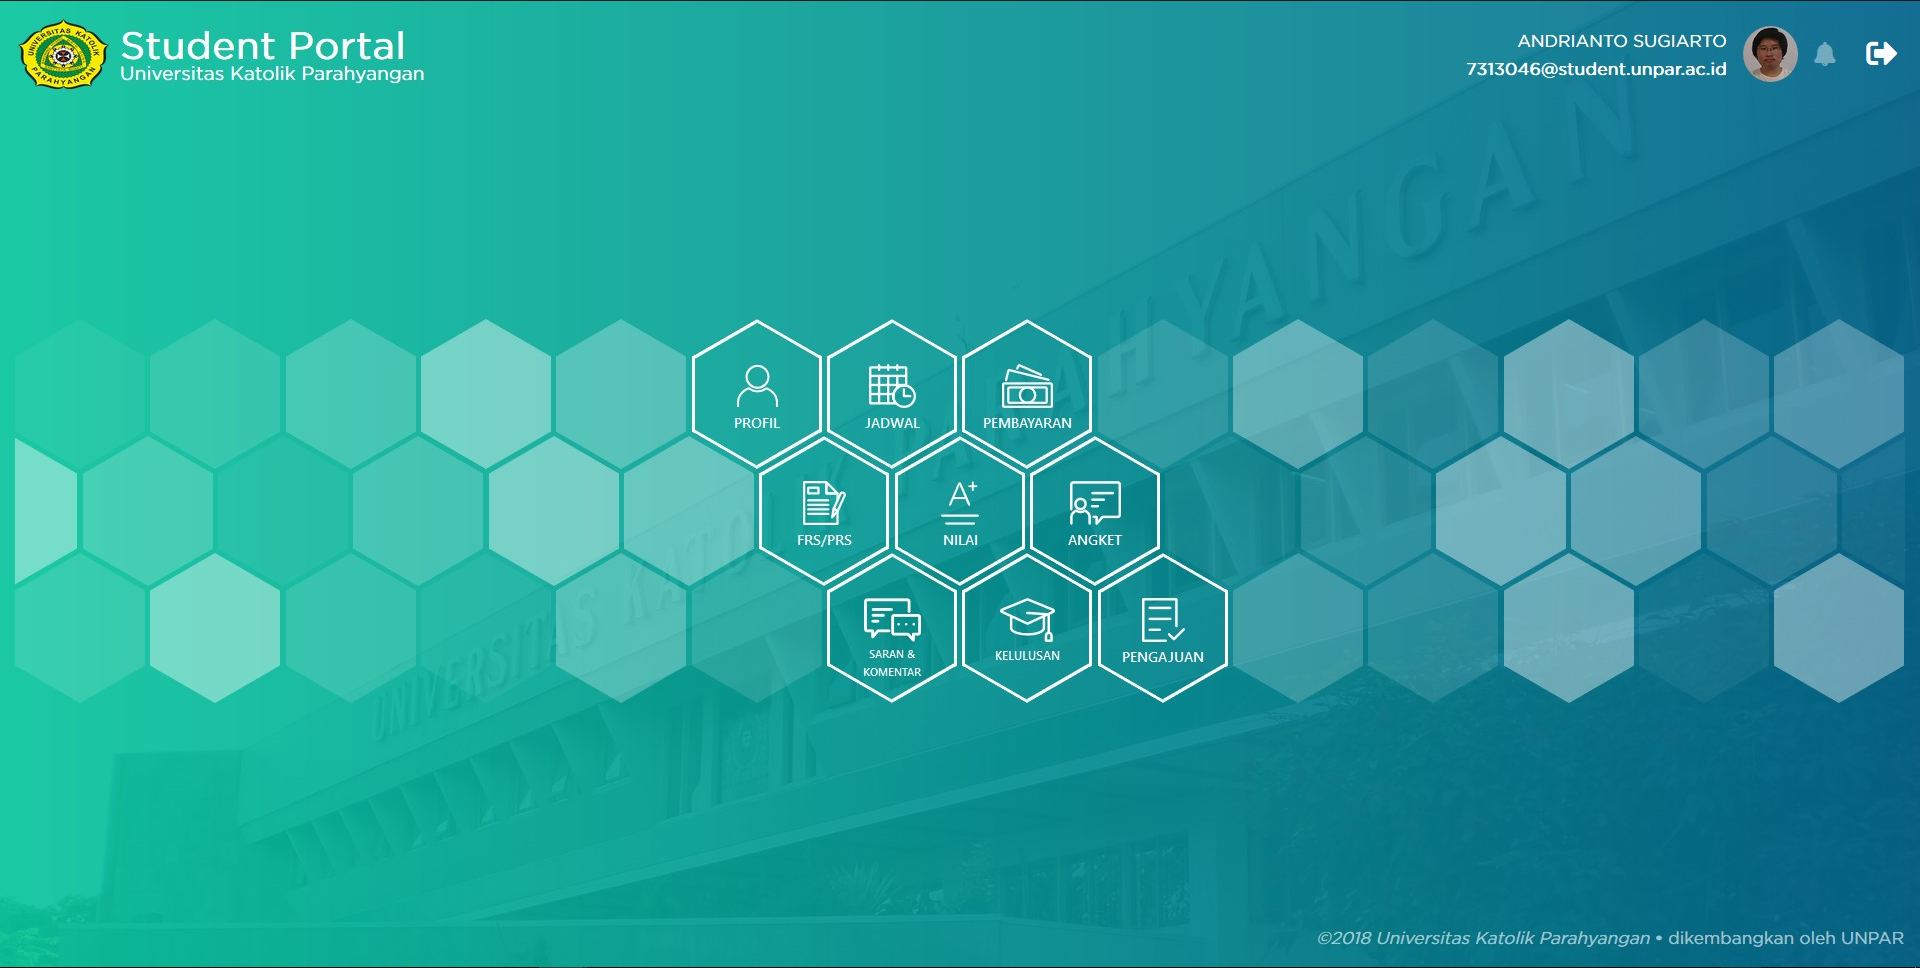
\includegraphics[scale=0.3]{Gambar/studentportal_home}
		\caption{Halaman Utama Portal Akademik Mahasiswa}
		\label{fig:studentportal_home}
	\end{figure}
	\item Menu Student Portal \\
	Bagian ini memuat fitur-fitur Student Portal yang terdiri dari:
	\begin{itemize}
		\item \textbf{Profil}, berisi tentang data diri masing-masing mahasiswa (Gambar \ref{fig:studentportal_profil}).
		\begin{figure}[H]
		\centering
		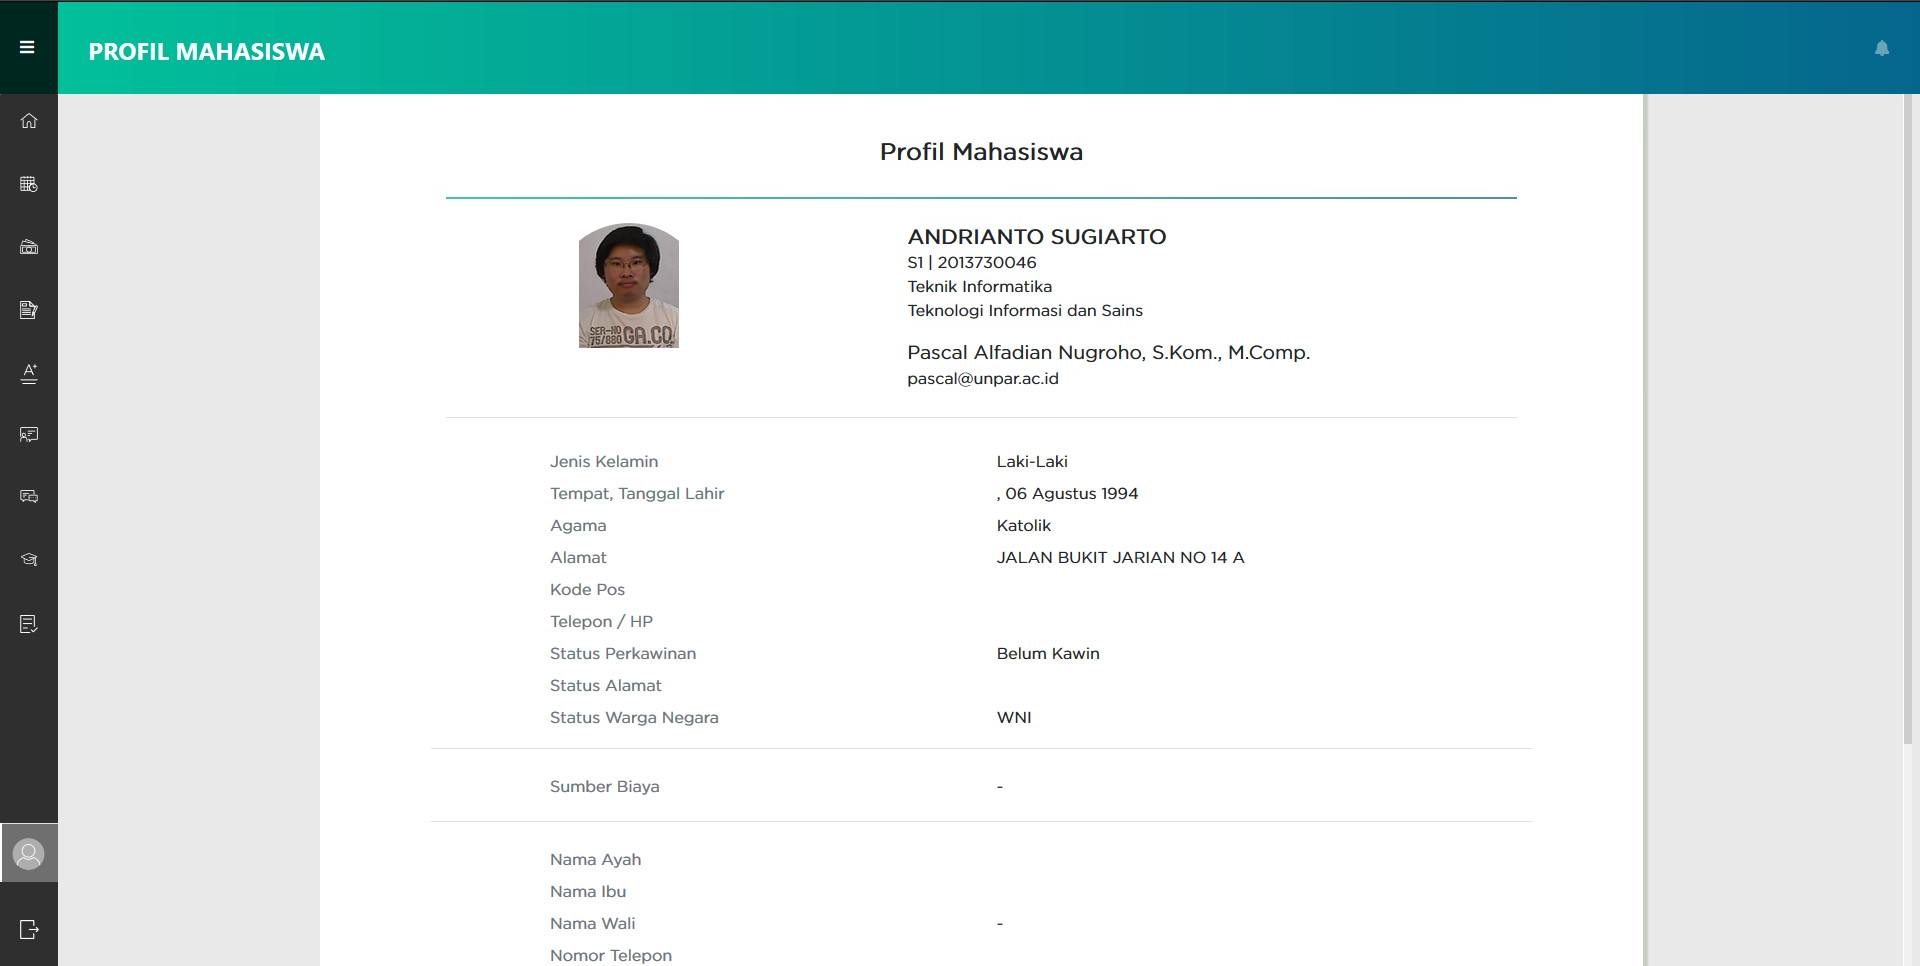
\includegraphics[scale=0.3]{Gambar/studentportal_profil}
		\caption{Tampilan Profil Student Portal}
		\label{fig:studentportal_profil}
		\end{figure}
		\item \textbf{Jadwal} \\
		Menu Jadwal terdiri dari submenu:
		\begin{itemize}
			\item Kuliah \\
			Submenu ini berisi tentang jadwal kuliah yang dapat disusun per semester dan terdapat 2 tampilan, yaitu tabel waktu dan tabel biasa (Gambar \ref{fig:studentportal_jadwal_kuliah_timetable} \& \ref{fig:studentportal_jadwal_kuliah_table})
			\begin{figure}[H]
			\centering
			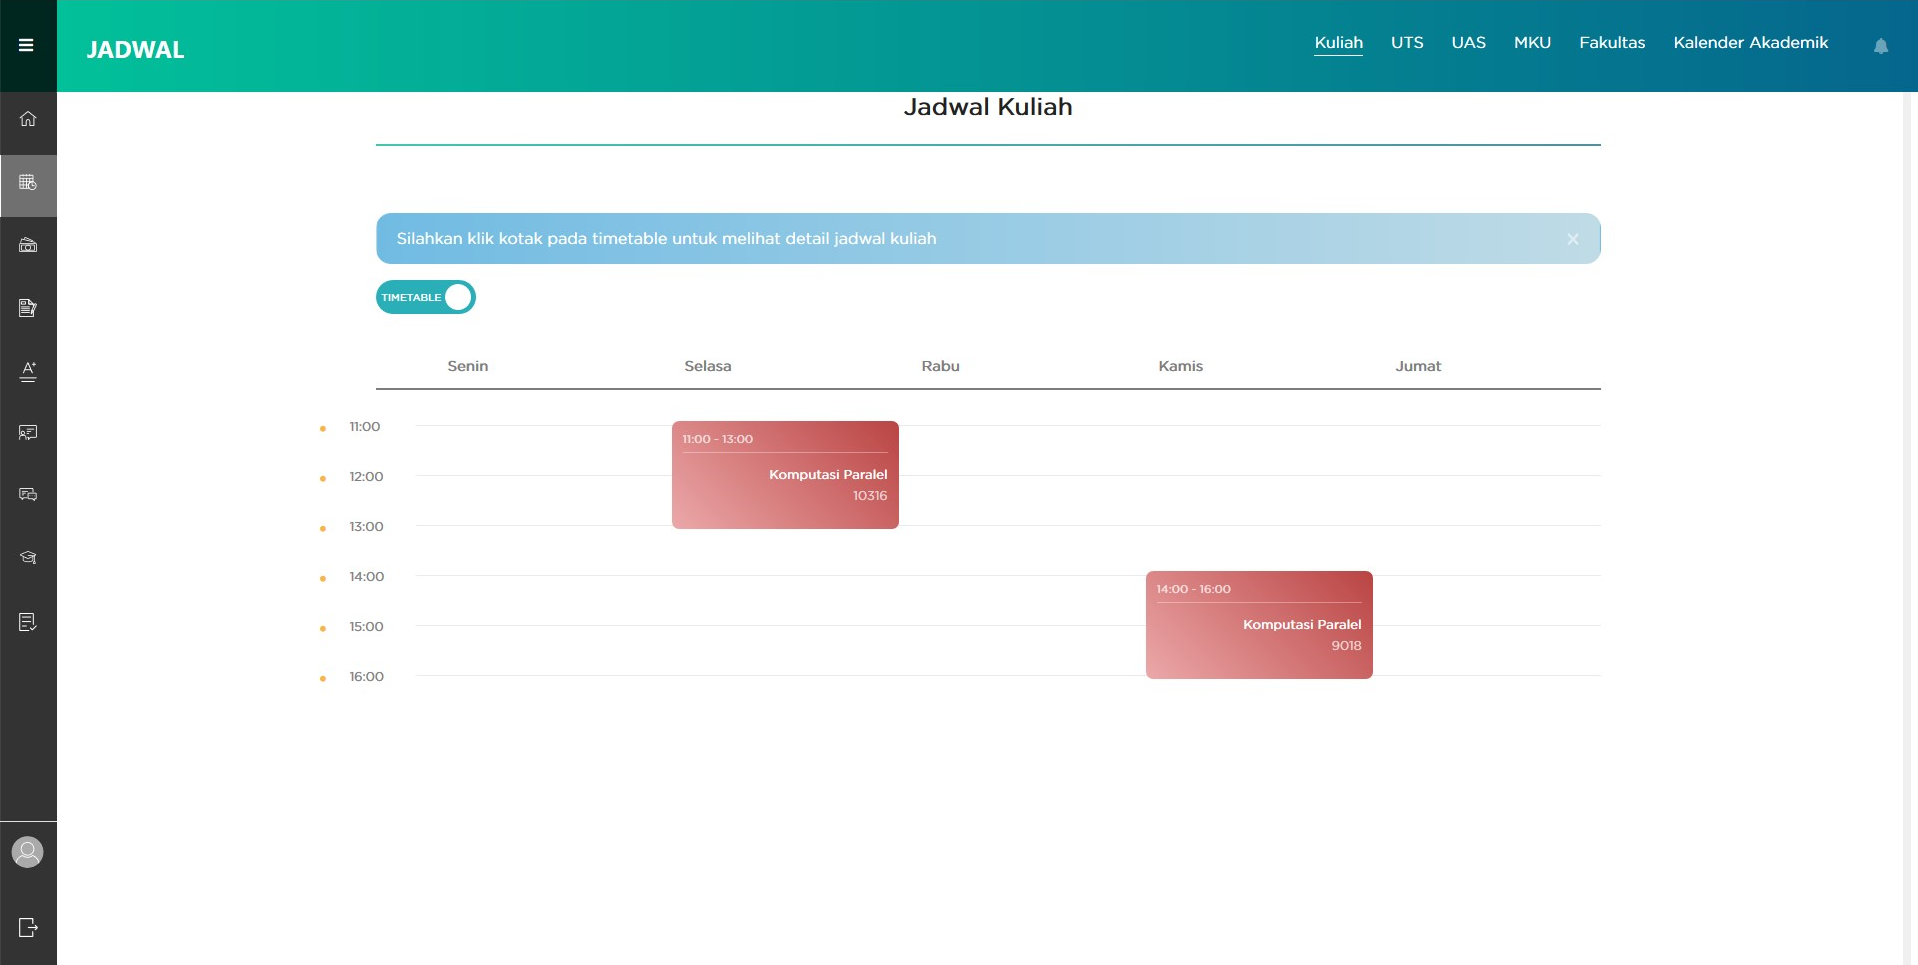
\includegraphics[scale=0.3]{Gambar/studentportal_jadwal_kuliah}
			\caption{Tampilan Jadwal Kuliah Dalam Tabel Waktu}
			\label{fig:studentportal_jadwal_kuliah_timetable}
			\end{figure}
			\begin{figure}[H]
			\centering
			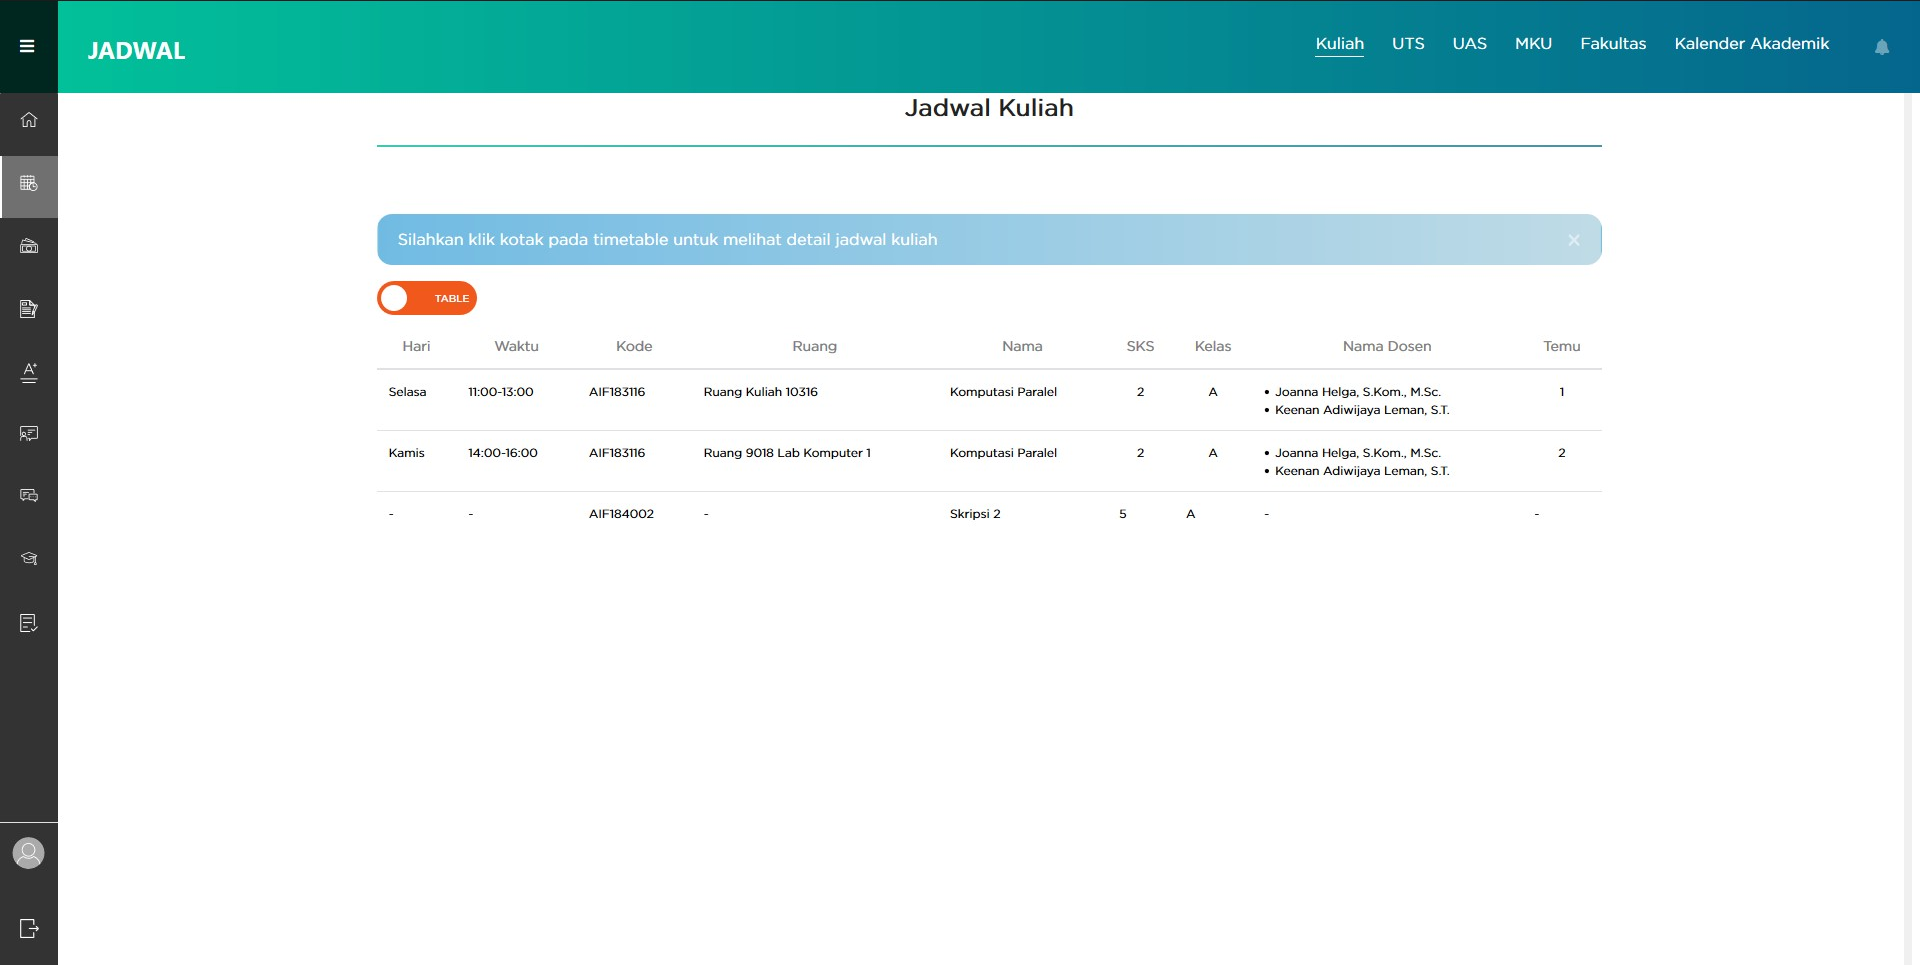
\includegraphics[scale=0.3]{Gambar/studentportal_jadwal_kuliah_table}
			\caption{Tampilan Jadwal Kuliah Tabel}
			\label{fig:studentportal_jadwal_kuliah_table}
			\end{figure}
			\item UTS \\
			Submenu ini berisi tentang UTS yang dapat disusun per semester (Gambar \ref{fig:studentportal_uts})
			\begin{figure}[H]
			\centering
			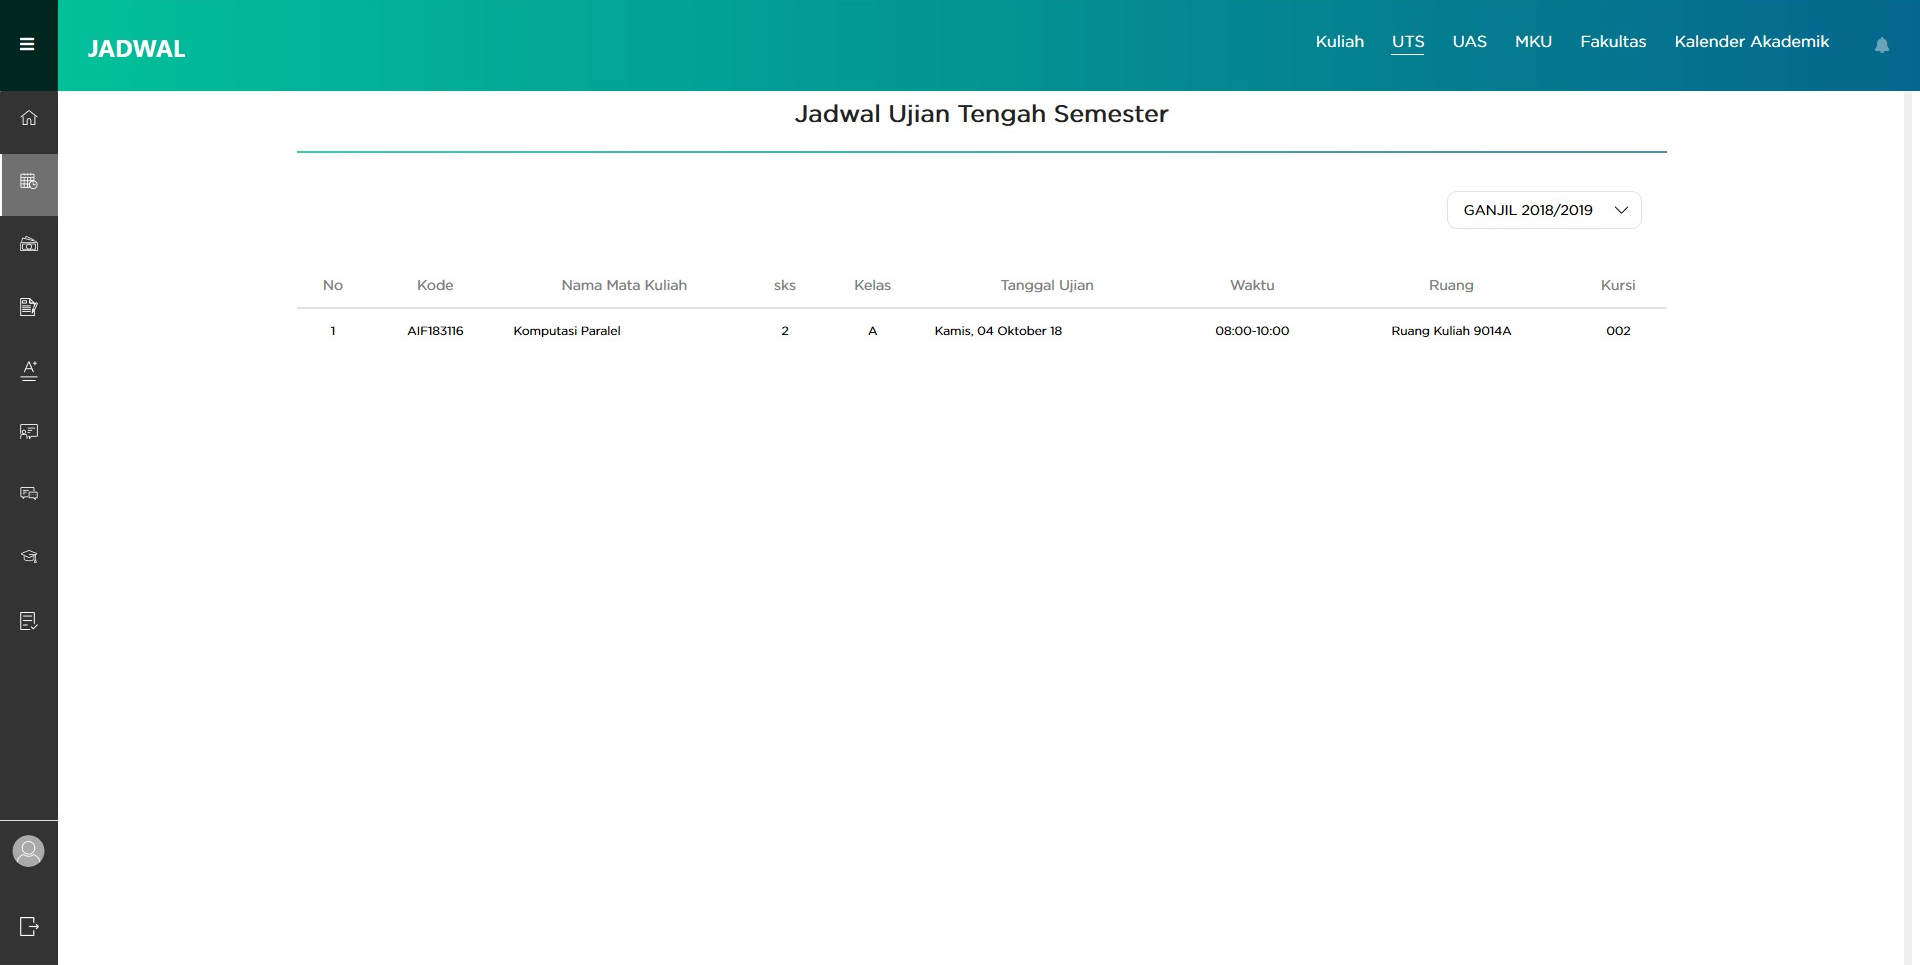
\includegraphics[scale=0.3]{Gambar/studentportal_jadwal_uts}
			\caption{Tampilan UTS}
			\label{fig:studentportal_uts}
			\end{figure}
			\item UAS \\
			Submenu ini berisi tentang UAS yang dapat disusun per semester (Gambar \ref{fig:studentportal_uas})
			\begin{figure}[H]
			\centering
			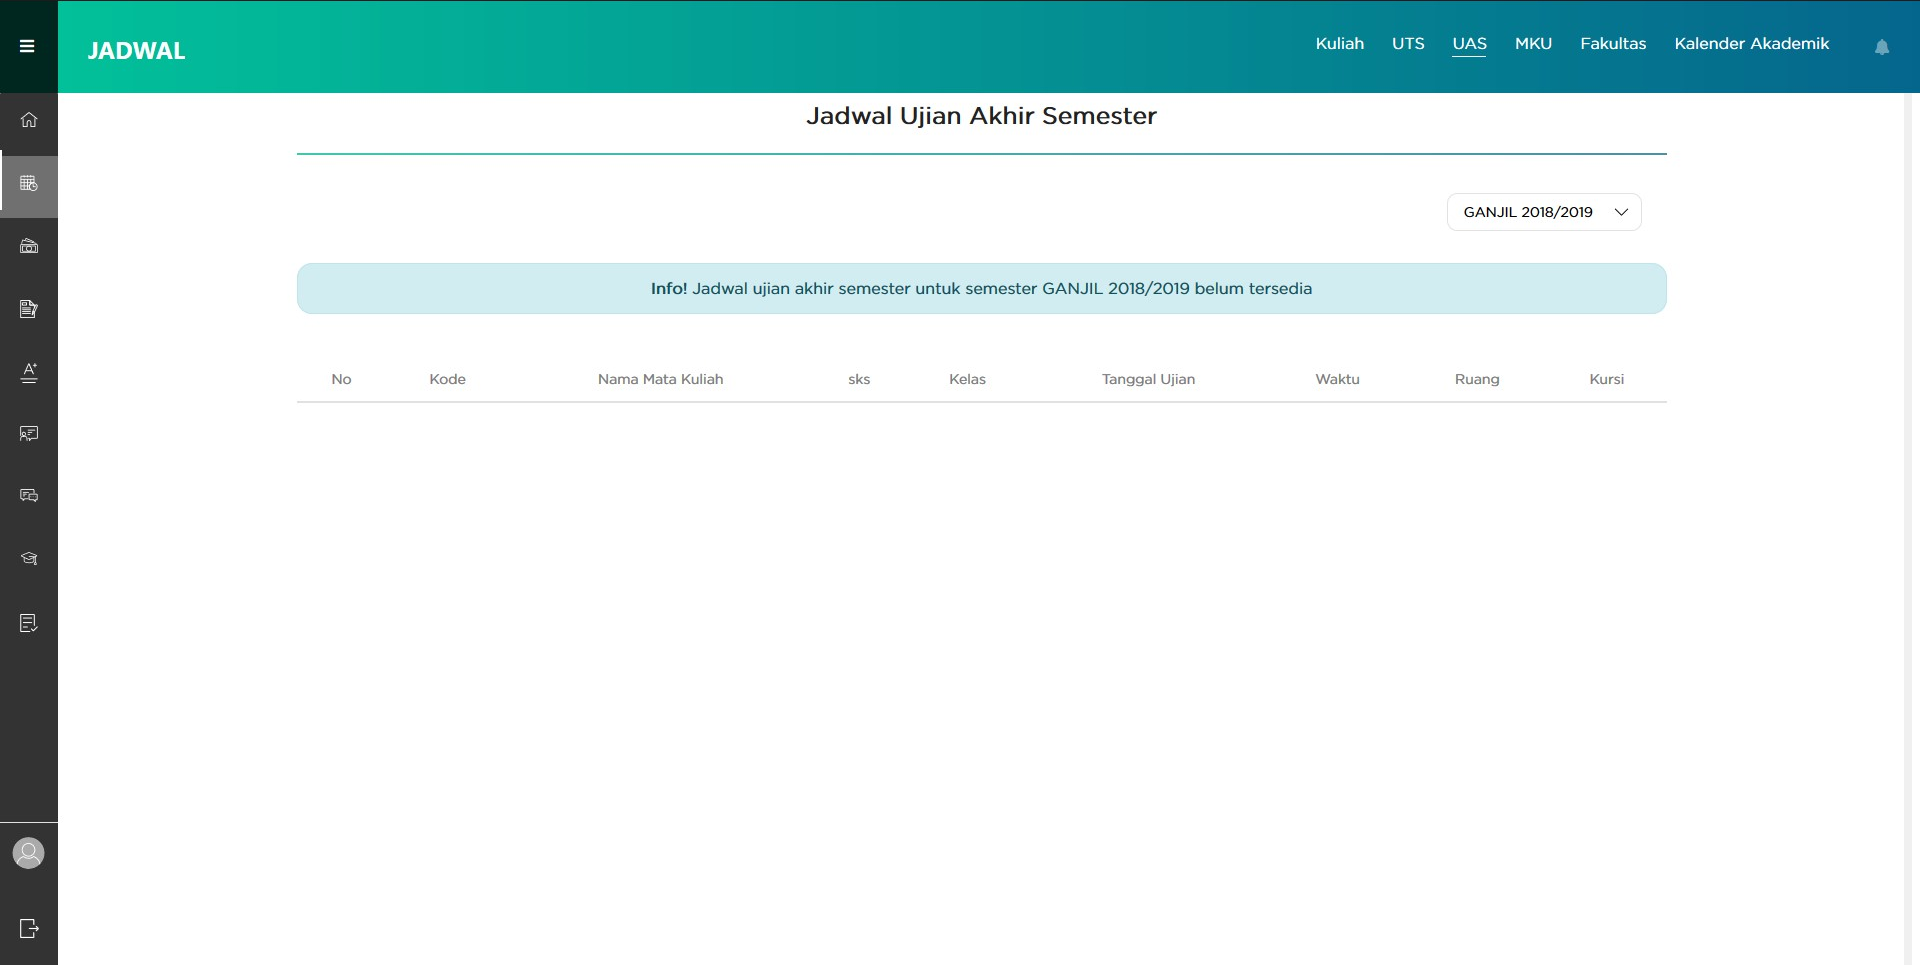
\includegraphics[scale=0.3]{Gambar/studentportal_jadwal_uas}
			\caption{Tampilan UAS}
			\label{fig:studentportal_uas}
			\end{figure}
			\item MKU \\
			Submenu ini menampilkan seluruh jadwal Mata Kuliah Umum (MKU) yang memberikan informasi tentang kelas-kelas yang dibuka oleh Pusat Kajian Humaniora (PKH) (Gambar \ref{fig:studentportal_jadwal_mku})
			\begin{figure}[H]
			\centering
			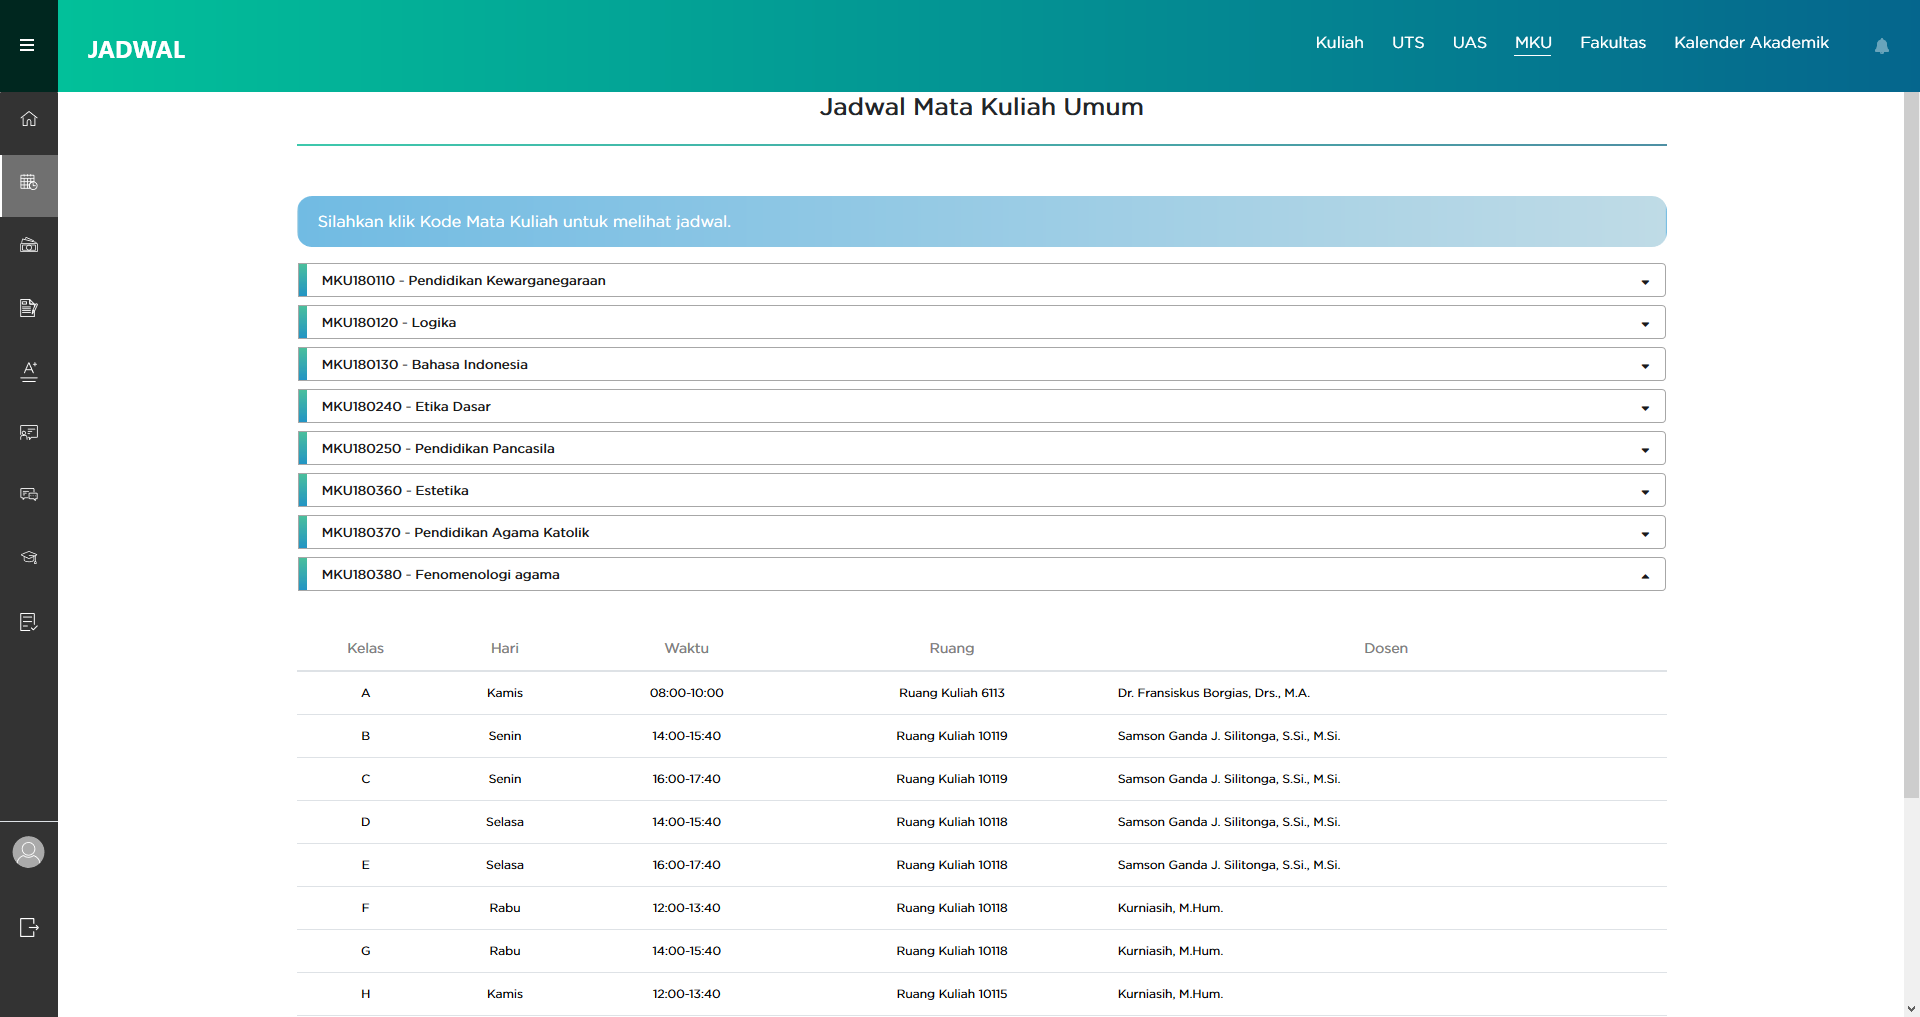
\includegraphics[scale=0.23]{Gambar/studentportal_jadwal_mku}
			\caption{Tampilan MKU}
			\label{fig:studentportal_jadwal_mku}
			\end{figure}
			\item Seluruh Fakultas \\
			Submenu ini memberikan informasi mengenai jadwal-jadwal yang ada diseluruh fakultas dan masih dalam pembangunan (Gambar \ref{fig:studentportal_jadwal_seluruh_fakultas})
			\begin{figure}[H]
			\centering
			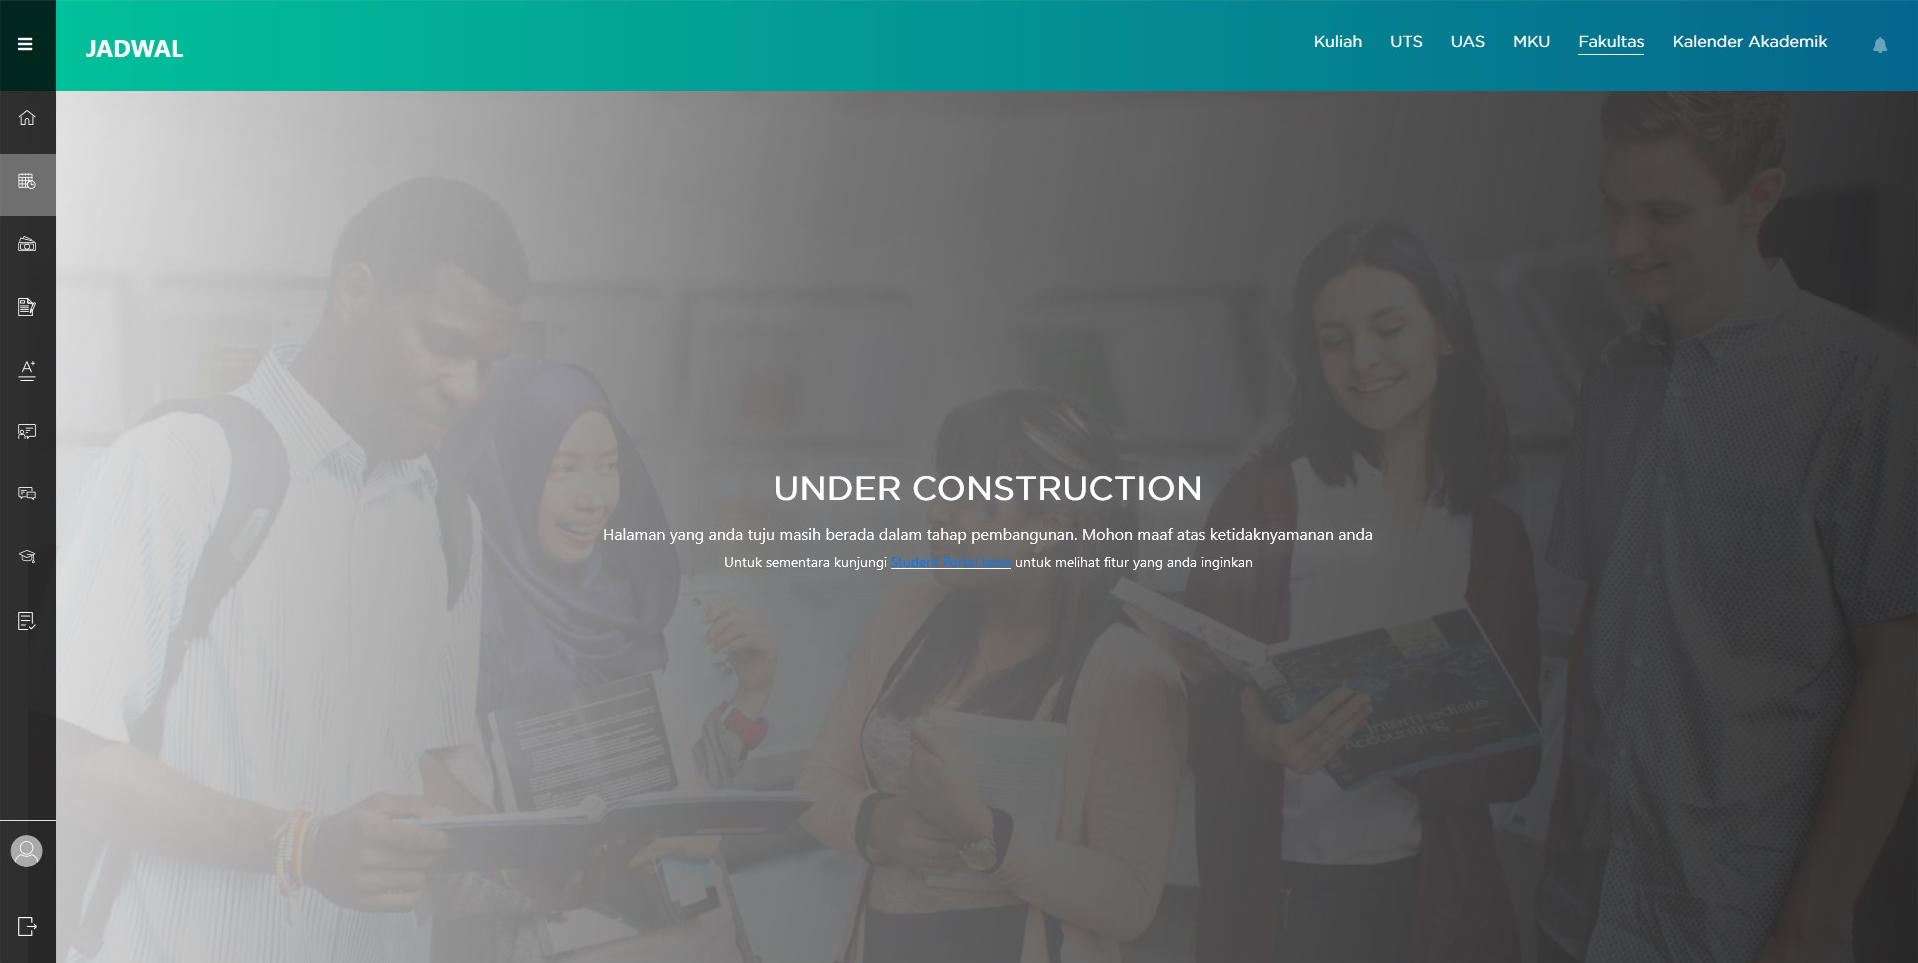
\includegraphics[scale=0.3]{Gambar/studentportal_seluruh_fakultas_under_construction}
			\caption{Tampilan Jadwal Seluruh Fakultas Under Construction}
			\label{fig:studentportal_jadwal_seluruh_fakultas}
			\end{figure}
			\item Kalender Akademik \\
			Submenu ini memberikan informasi kalender akademik UNPAR dan masih dalam pembangunan.
		\end{itemize}
		\item \textbf{Pembayaran Uang Kuliah} \\
		Menu ini berfungsi untuk melihat data tagihan pembayaran uang kuliah, riwayat pembayaran, dan keterangan cara-cara pembayaran uang kuliah (Gambar \ref{fig:studentportal_pembayaran_kuliah}).
		\begin{figure}[H]
			\centering
			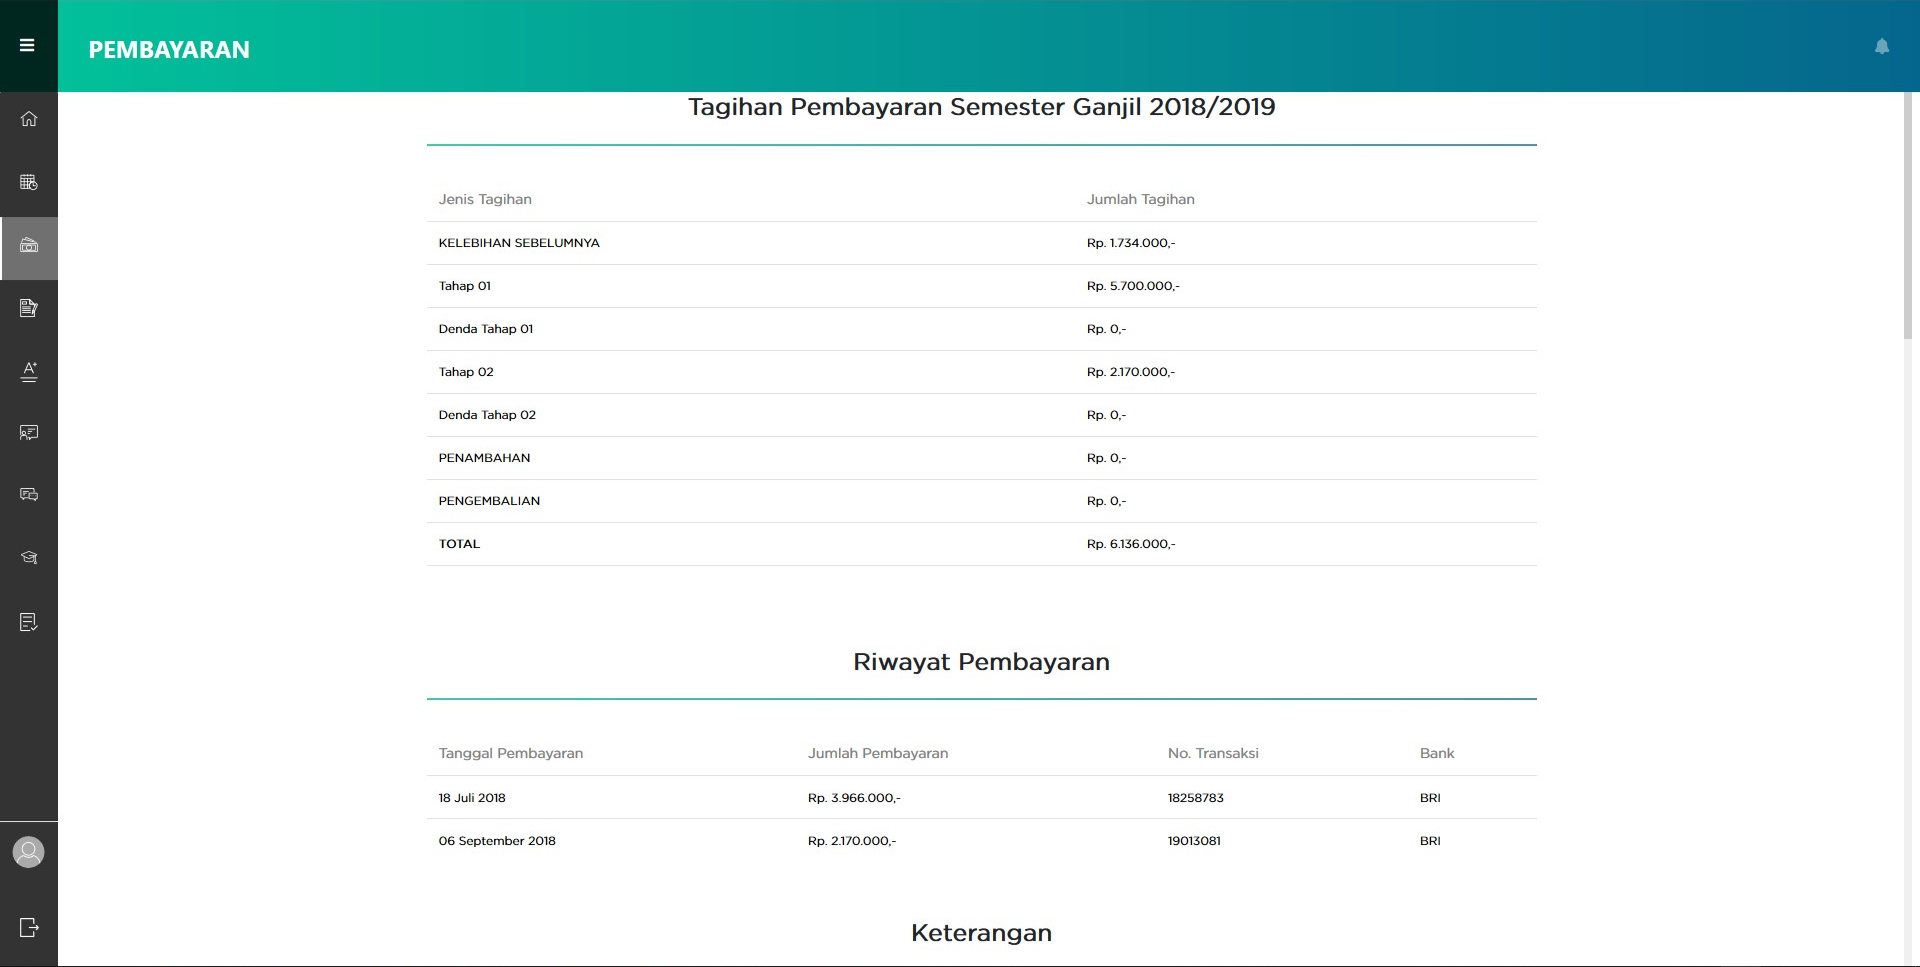
\includegraphics[scale=0.3]{Gambar/studentportal_pembayaran_kuliah}
			\caption{Tampilan Pembayaran Kuliah}
			\label{fig:studentportal_pembayaran_kuliah}
		\end{figure}
		\item FRS/PRS
		Menu FRS/PRS terdiri dari submenu:
		\begin{itemize}
			\item FRS/PRS \\
			Digunakan sebagai formulir pengisian rencana studi awal (FRS), perubahan rencana studi(PRS) dan menampilkan informasi mata kuliah yang telah diambil saat FRS atau PRS (Gambar \ref{fig:studentportal_frs_prs}).
			\begin{figure}[H]
				\centering
				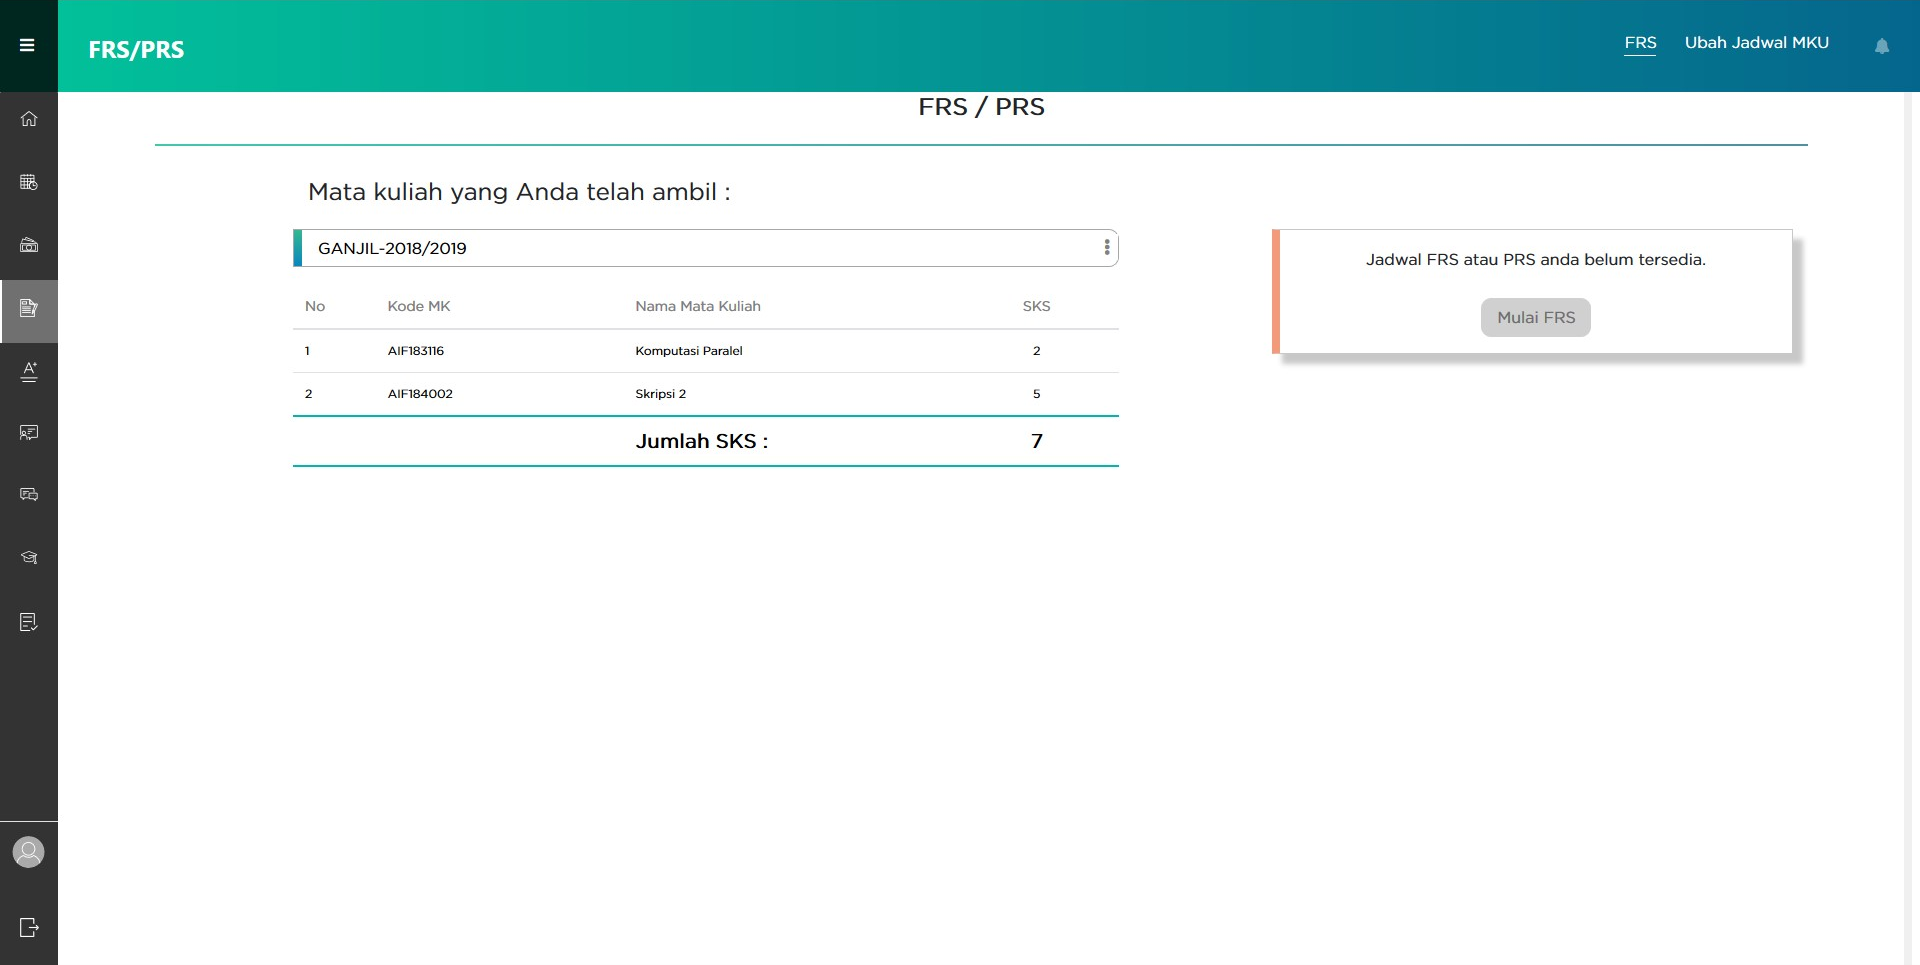
\includegraphics[scale=0.3]{Gambar/studentportal_frs_prs}
				\caption{Tampilan FRS/PRS}
				\label{fig:studentportal_frs_prs}
			\end{figure}
			\item Ubah Jadwal MKU \\
			Mahasiswa dapat mengubah jadwal kelas MKU (Gambar \ref{fig:studentportal_ubah_jadwal_mku}).
			\begin{figure}[H]
				\centering
				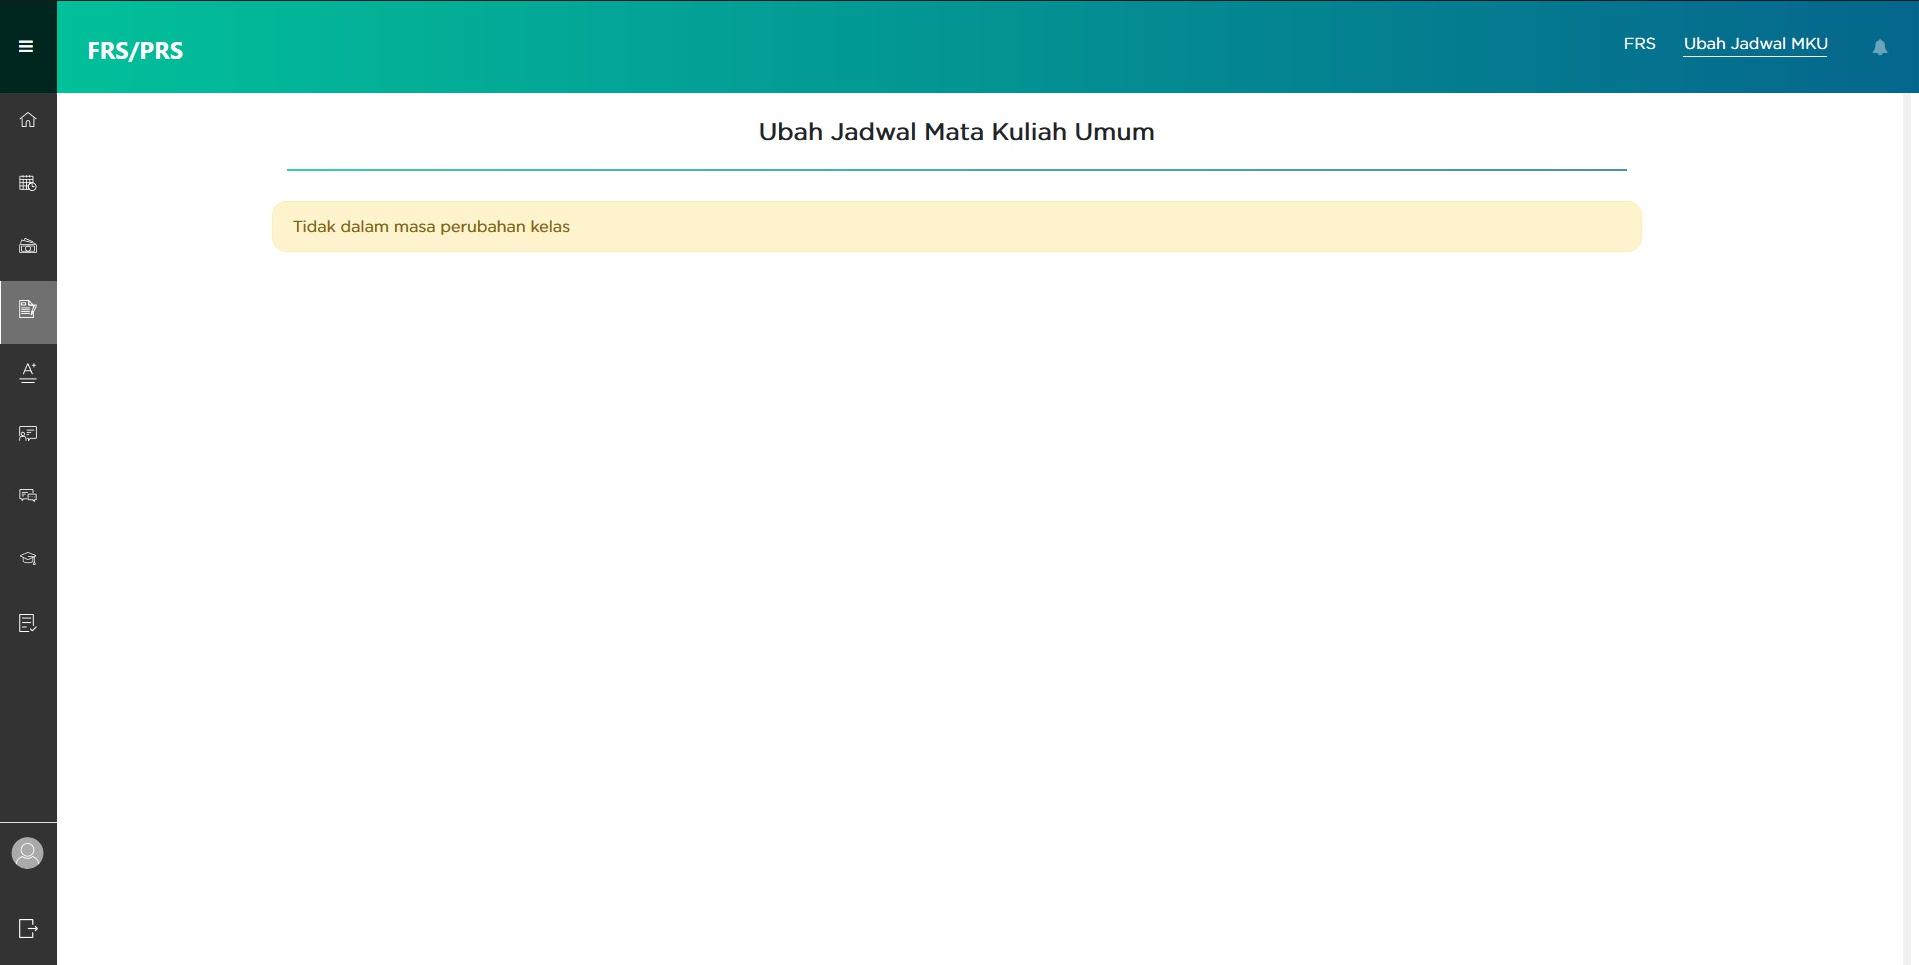
\includegraphics[scale=0.3]{Gambar/studentportal_ubah_jadwal_mku}
				\caption{Tampilan Ubah Jadwal MKU}
				\label{fig:studentportal_ubah_jadwal_mku}
			\end{figure}
		\end{itemize}
		\item \textbf{Nilai}
		Menu Nilai terdiri dari submenu:
		\begin{itemize}
			\item Nilai per Semester \\
			Submenu ini menampilkan informasi nilai per semester. Mahasiswa dapat melihat nilai sesuai dengan semester yang dipilih (Gambar \ref{fig:studentportal_nilai_per_semester}).
			\begin{figure}[H]
				\centering
				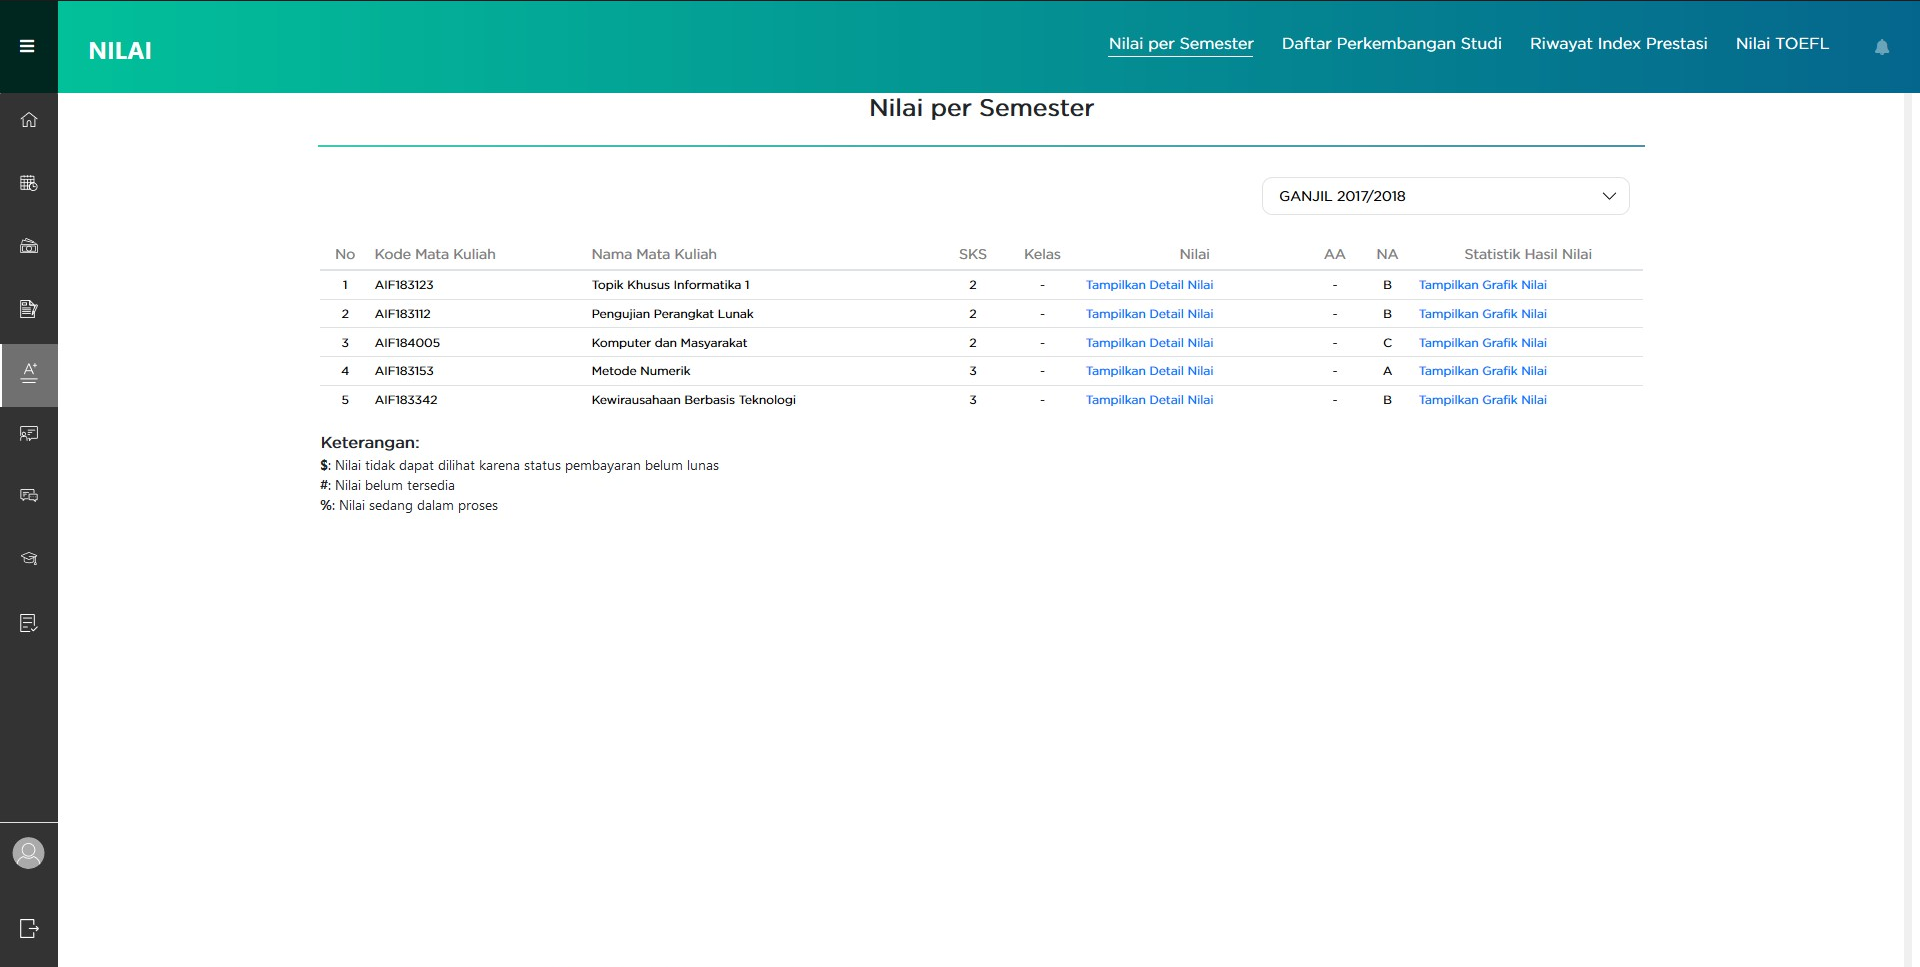
\includegraphics[scale=0.3]{Gambar/studentportal_nilai_per_semester}
				\caption{Tampilan Nilai Per Semester}
				\label{fig:studentportal_nilai_per_semester}
			\end{figure}
			\item Daftar Perkembangan Studi \\
			Seluruh riwayat mata kuliah dan nilai yang pernah ditempuh di submenu ini (Gambar \ref{fig:studentportal_dps_1}). Pada bagian bawah halaman, terdapat statistik nilai dan indeks perstasi (Gambar \ref{fig:studentportal_dps_2}).
			\begin{figure}[H]
				\centering
				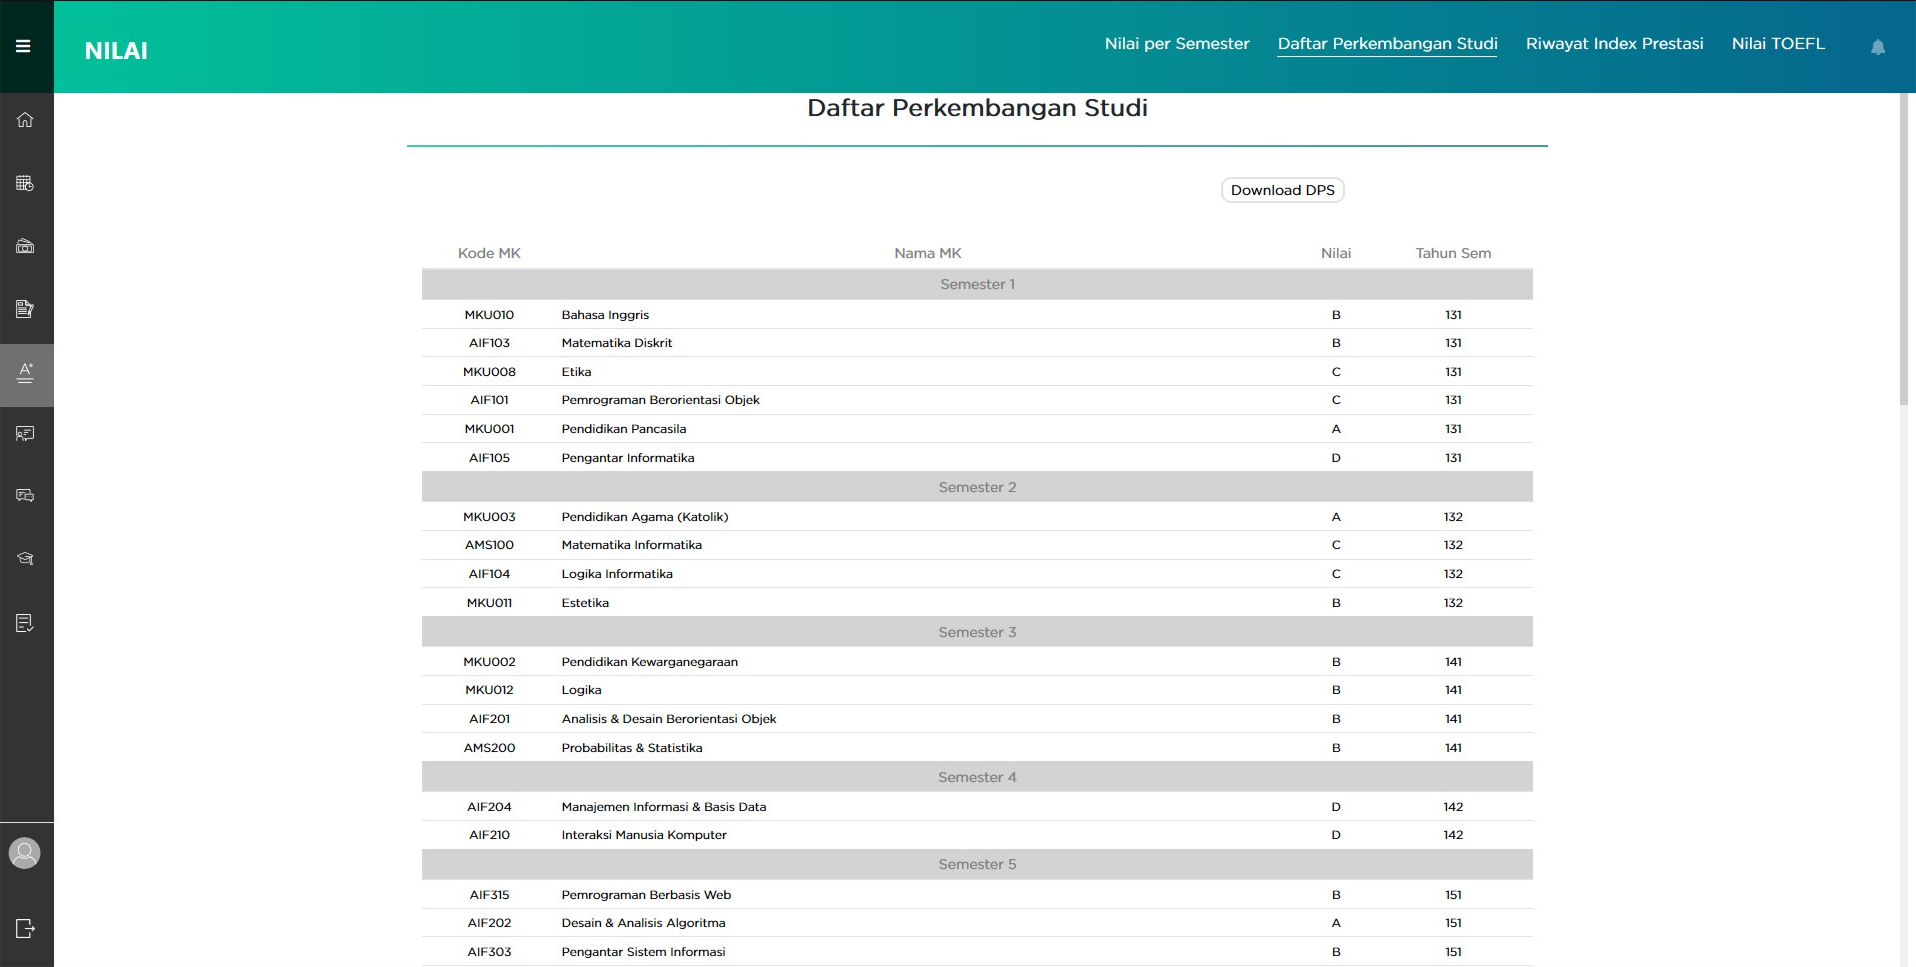
\includegraphics[scale=0.3]{Gambar/studentportal_dps_1}
				\caption{Tampilan Daftar Perkembangan Studi}
				\label{fig:studentportal_dps_1}
			\end{figure}
			\begin{figure}[H]
				\centering
				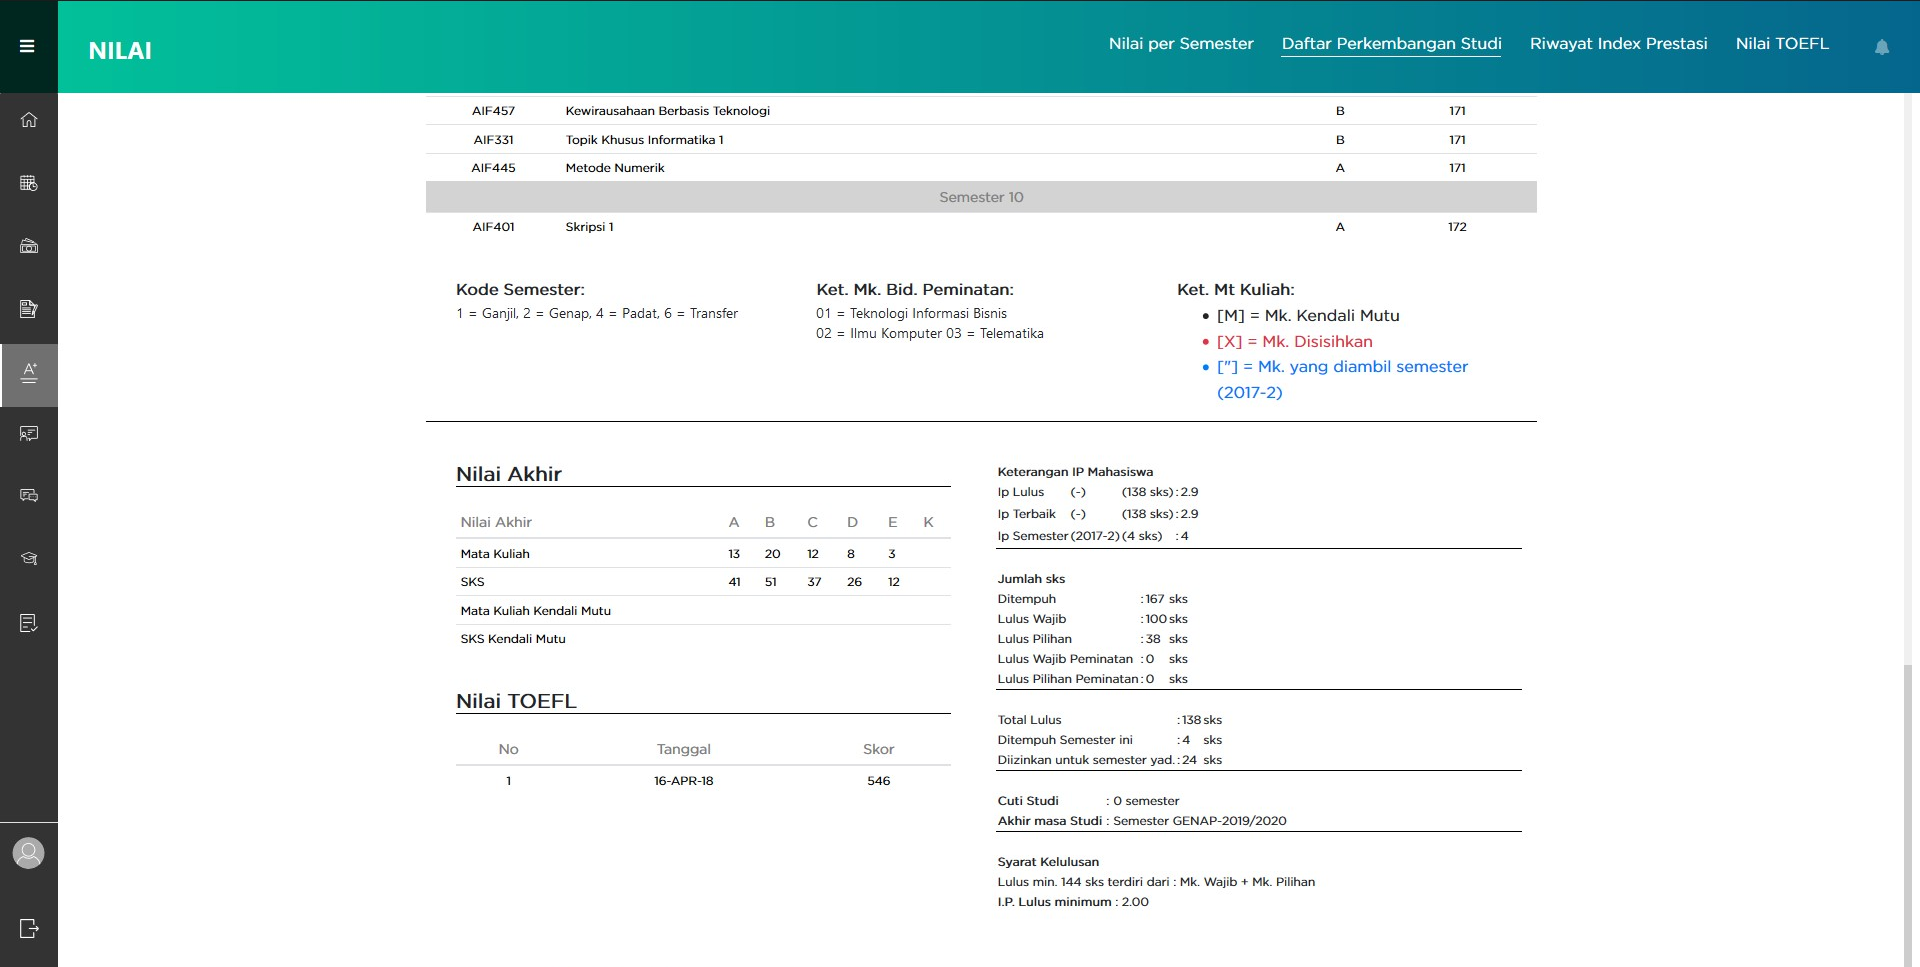
\includegraphics[scale=0.3]{Gambar/studentportal_dps_2}
				\caption{Tampilan Statistik Nilai dan IP}
				\label{fig:studentportal_dps_2}
			\end{figure}
			\item Riwayat Index Prestasi \\
			Menampilkan daftar riwayat Indeks Prestasi Semester(IPS) dan Indeks Prestasi Kumulatif(IPK) setiap semester (Gambar \ref{fig:studentportal_rip_2}). Tampilan ini juga dilengkapi dengan grafik perkembangan (Gambar \ref{fig:studentportal_rip_1})
			\begin{figure}[H]
				\centering
				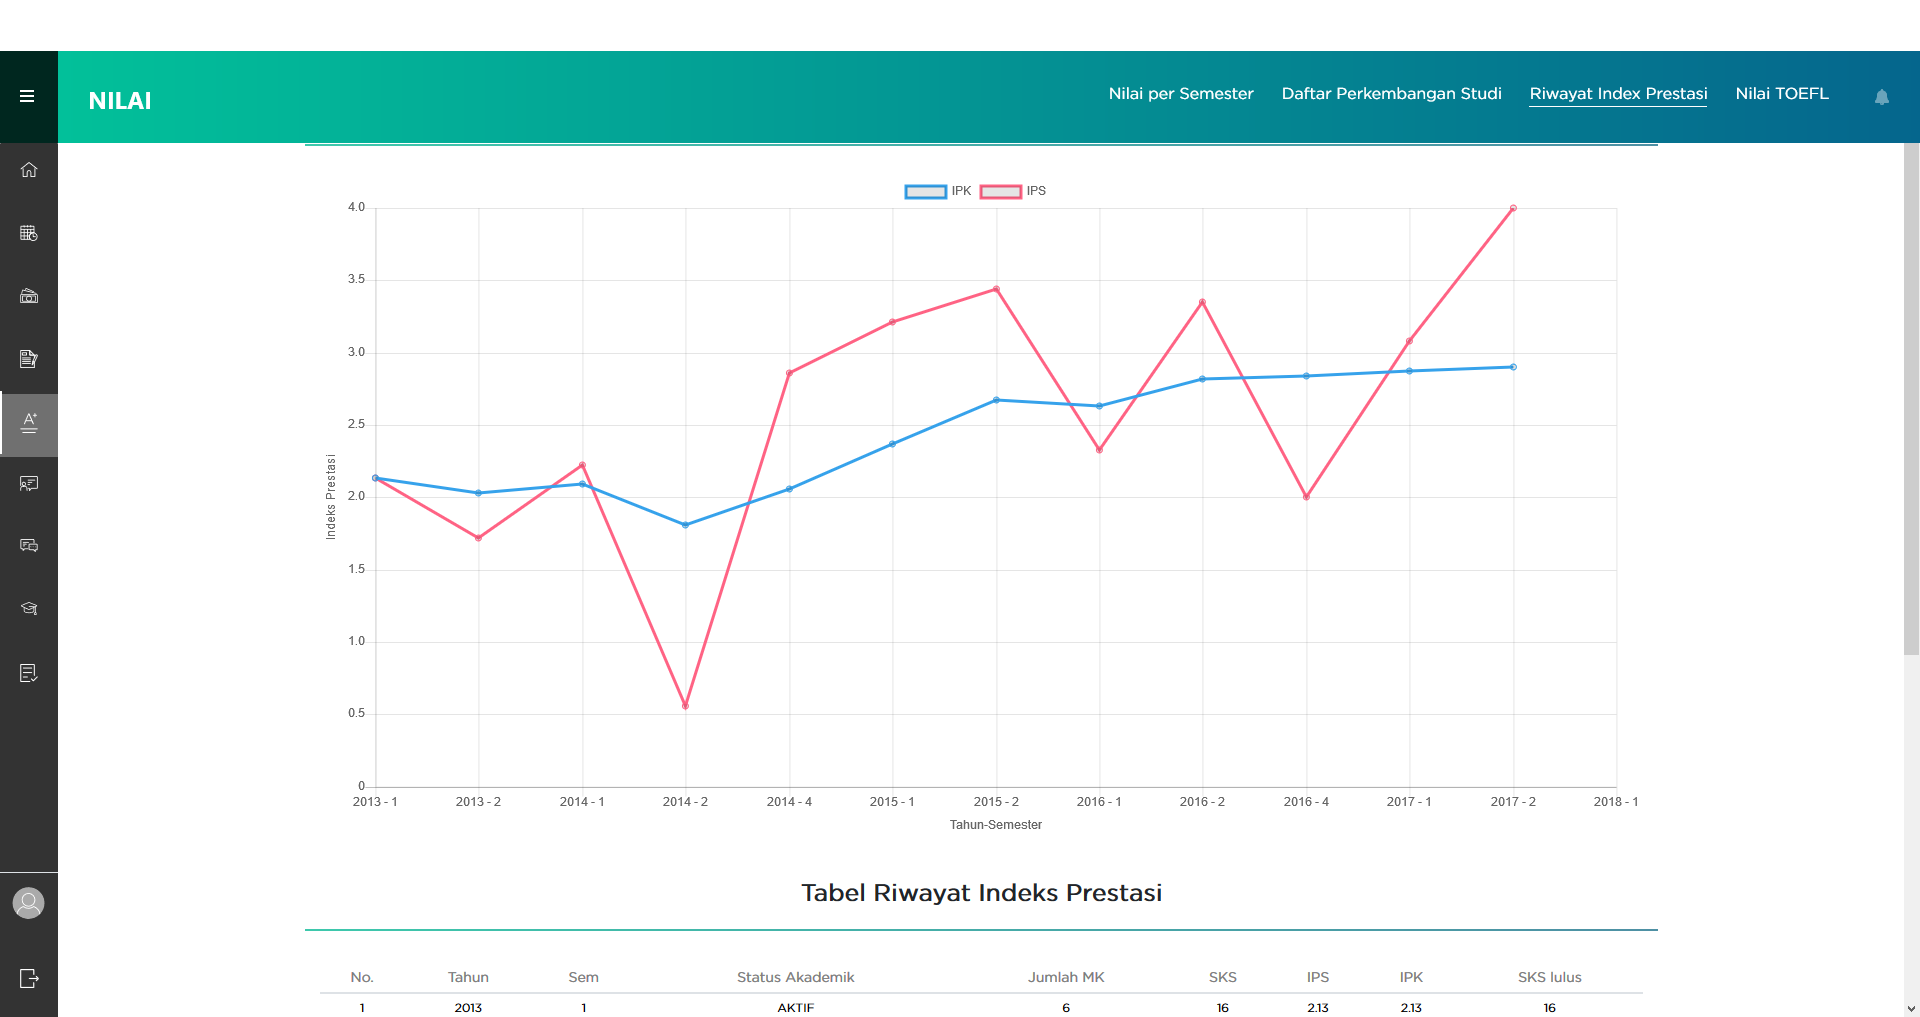
\includegraphics[scale=0.23]{Gambar/studentportal_rip}
				\caption{Tampilan Grafik Riwayat Index Prestasi}
				\label{fig:studentportal_rip_1}
			\end{figure}
			\begin{figure}[H]
				\centering
				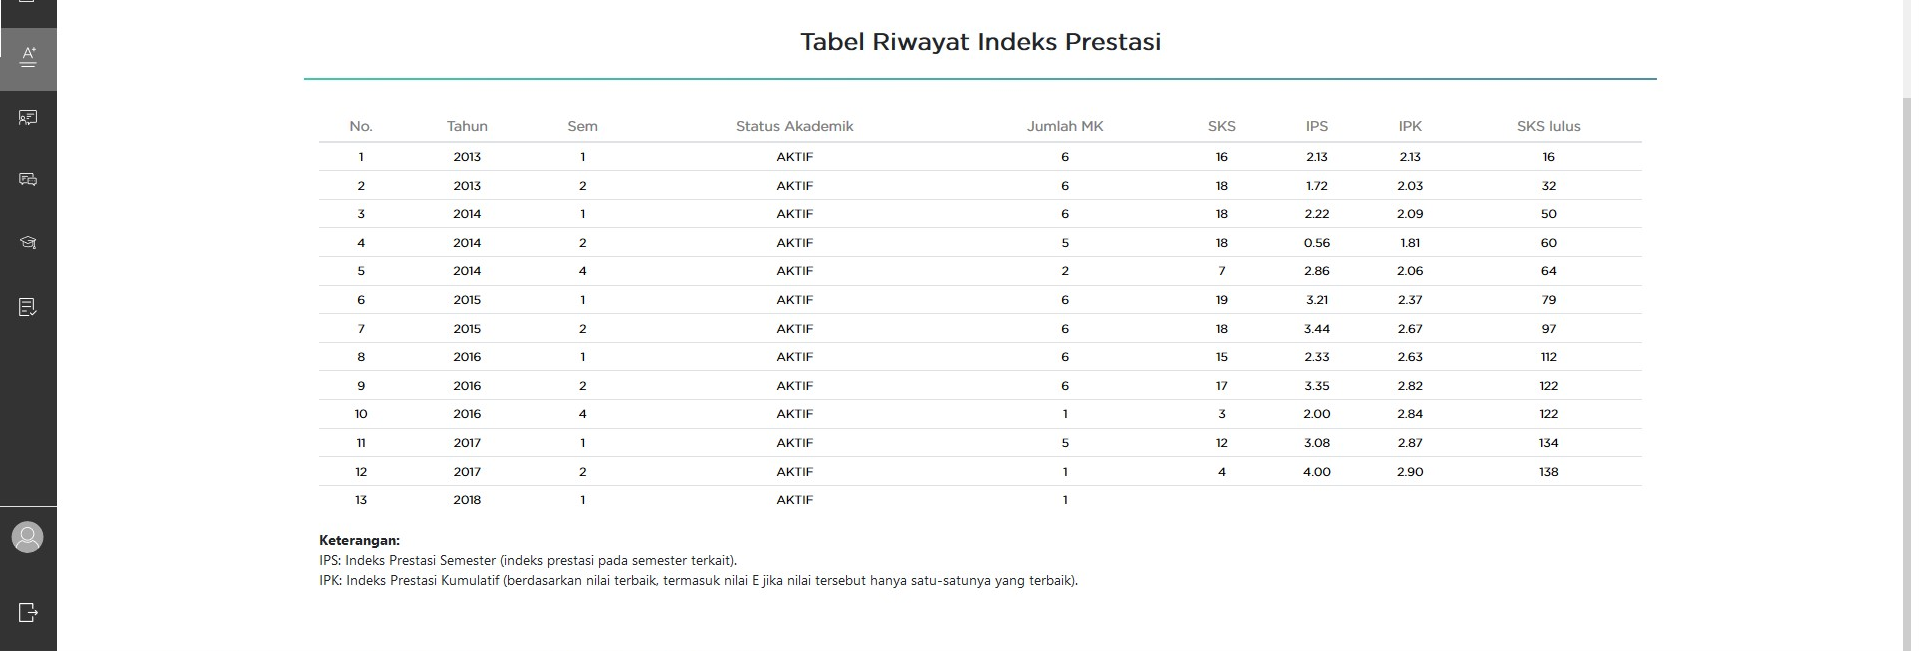
\includegraphics[scale=0.3]{Gambar/studentportal_rip_2}
				\caption{Tampilan Daftar Riwayat Indeks Prestasi}
				\label{fig:studentportal_rip_2}
			\end{figure}
			\item Nilai TOEFL \\
			Menampilkan daftar riwayat skor dan detail skor \textit{Test of English as Foreign Language} (TOEFL) yang pernah ditempuh (Gambar \ref{fig:studentportal_nilai_toefl}).
			\begin{figure}[H]
				\centering
				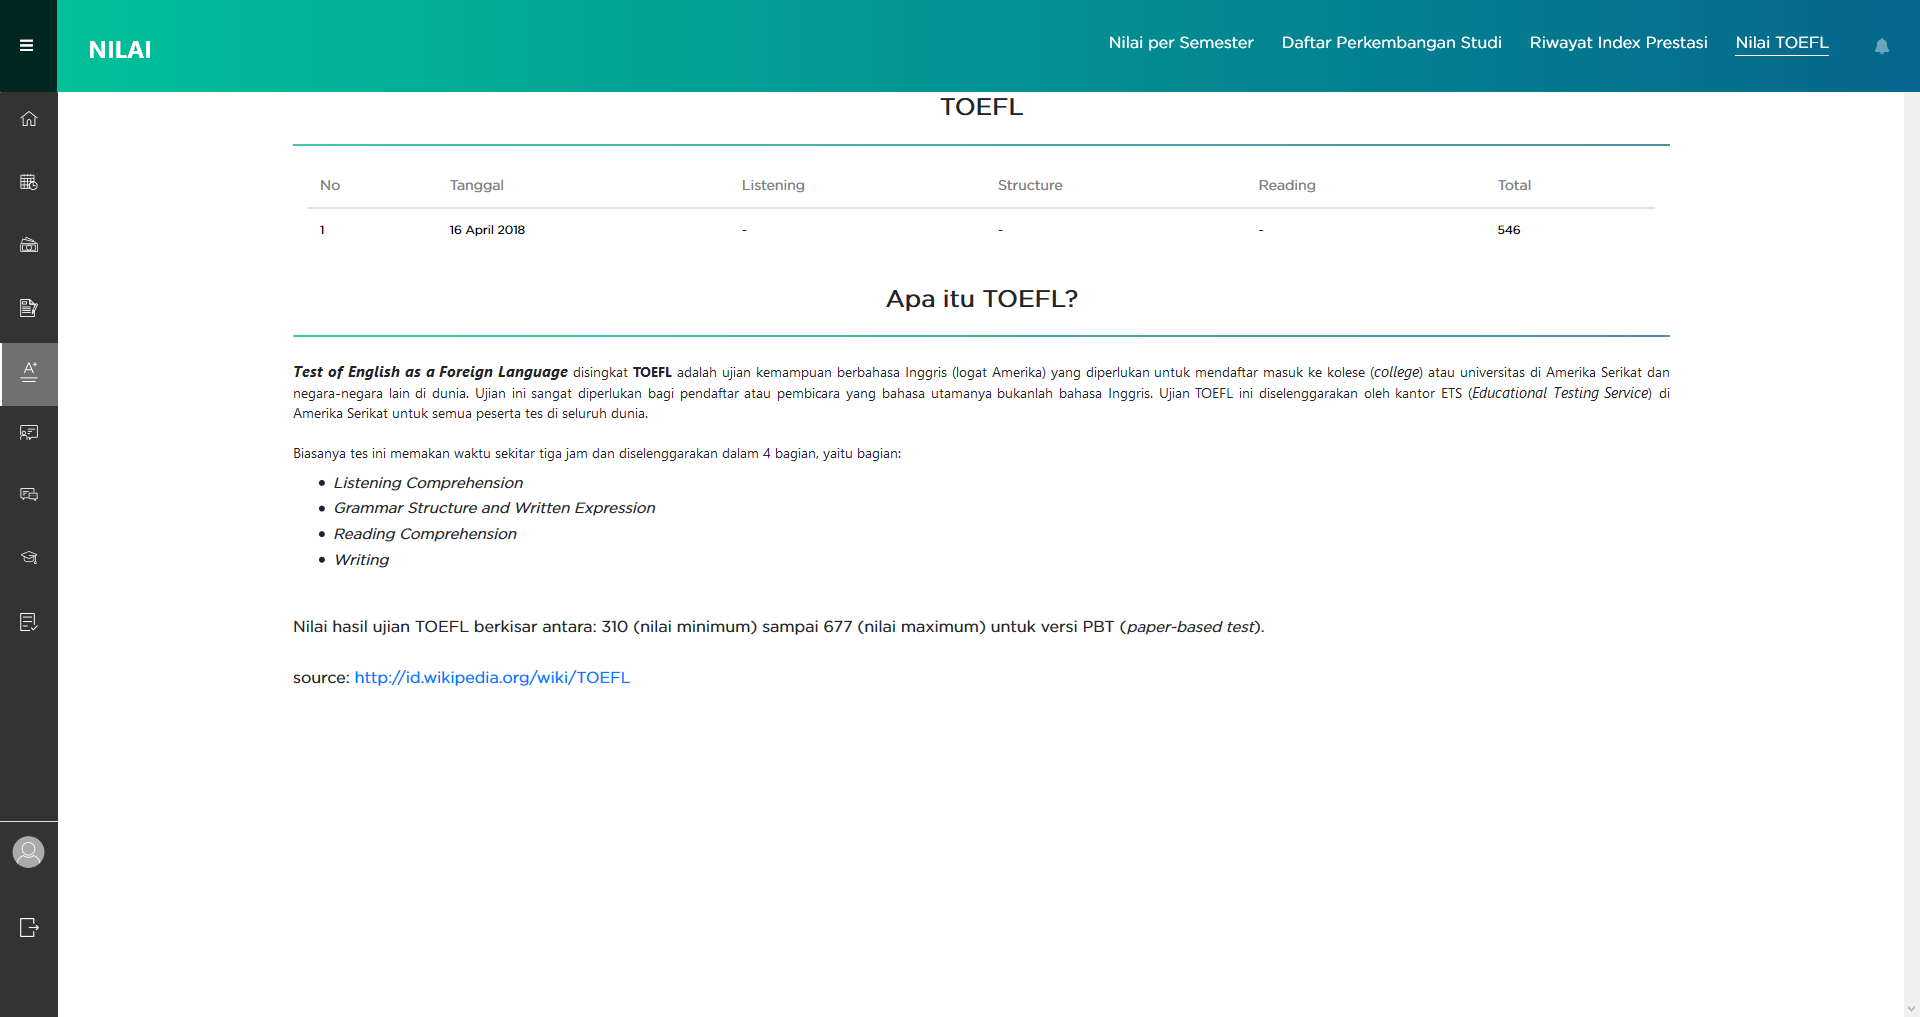
\includegraphics[scale=0.23]{Gambar/studentportal_nilai_toefl}
				\caption{Tampilan Daftar Perkembangan Studi}
				\label{fig:studentportal_nilai_toefl}
			\end{figure}
		\end{itemize}
		\item Menu Angket, Kelulusan, dan Pengajuan \\
		Menu Angket, Kelulusan, dan Pengajuan dalam tahap pembangunan.
		\item Saran dan Komentar \\
		Menu ini akan membuka link ke \url{https://suaramahasiswa.unpar.ac.id/}.
	\end{itemize}
	\item Pengumuman \\
	Menampilkan pengumuman dibagi jadi 2, yaitu pengumuman pribadi dan pengumuman prodi (Gambar \ref{fig:studentportal_pengumuman}).
	\begin{figure}[H]
		\centering
		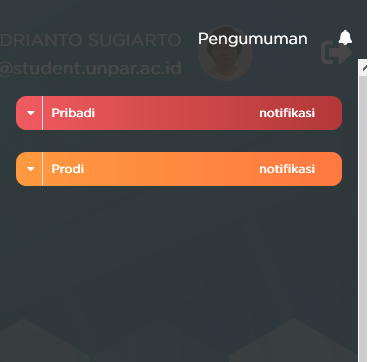
\includegraphics[scale=0.75]{Gambar/studentportal_pengumuman}
		\caption{Tampilan Pengumuman}
		\label{fig:studentportal_pengumuman}
	\end{figure}
\end{enumerate}

\section{Analisis Sistem IFStudentPortal}

\subsection{Aristektur IFStudentPortal}
	\begin{figure}[H]
			\centering
			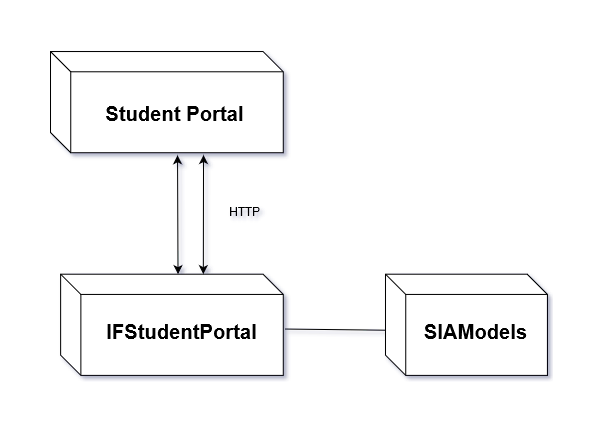
\includegraphics[scale=0.5]{Gambar/arsitektur_ifstudentportal}
			\caption{Aristektur IFStudentPortal} 
			\label{fig:3_ars_portal}
		\end{figure}
Aristektur IFStudentPortal dapat dilihat pada Gambar \ref{fig:3_ars_portal}. IFStudentPortal akan melakukan \textit{http} ke Student Portal UNPAR untuk mendapatkan data untuk setiap kebutuhan dari masing-masing fitur yang ada. Untuk pengambilan data secara langsung dari Student Portal UNPAR dilakukan menggunakan \textit{library} jsoup. Data yang telah didapat dari Student Portal UNPAR diolah ke dalam SIAModels kemudian akan ditampilkan sesuai dengan fitur-fitur yang ada pada IFStudentPortal.
 
\subsection{\textit{Use Case} IFStudentPortal}
\subsubsection{Diagram \textit{Use Case}}
	\begin{figure}[H]
			\centering
			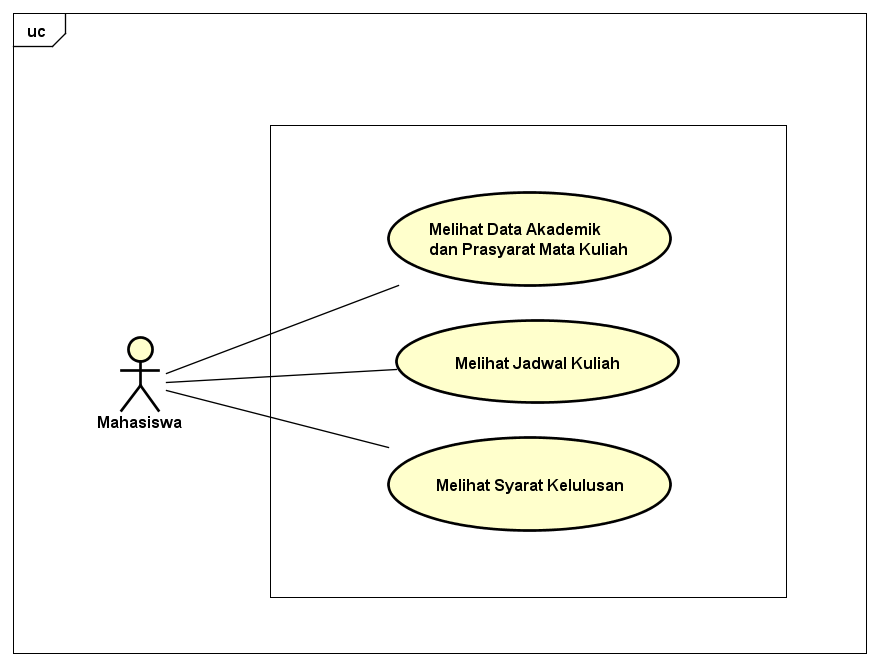
\includegraphics[scale=0.5]{Gambar/usecasediagram_ifstudentportal}
			\caption{Diagram \textit{Use Case} IFStudentPortal} 
			\label{fig:3_usecase_diagram}
		\end{figure}
Diagram \textit{use case} IFStudentPortal (Gambar \ref{fig:3_usecase_diagram}) terdapat 3 \textit{use case} yang menjadi 3 fitur utama dari IFStudentPortal, yaitu:
\begin{itemize}
	\item \textbf{Melihat Data Akademik dan Prasyarat Mata Kuliah}, mahasiswa dapat melihat mata kuliah yang dibuka pada semester terkini apakah sudah memenuhi prasyarat atau tidak. Mahasiswa juga dapat melihat IPS, IPK, IP Lulus, IP N. Terbaik, SKS lulus, dan Nilai TOEFL yang ter-\textit{update}.
	\item \textbf{Melihat Jadwal Kuliah}, Mahasiswa dapat melihat jadwal kuliah yang sudah tersusun dan terurut berdasarkan hari.
	\item \textbf{Melihat Syarat Kelulusan}, Mahasiswa dapat melihat syarat kelulusan yang belum terpenuhi untuk lulus dari Program Studi Teknik Informatika. Syarat Kelulusan mencakup mata kuliah wajib apa saja yang belum lulus dan sks yang kurang untuk bisa lulus.
\end{itemize}
\subsubsection{Skenario \textit{Use Case}}
\begin{enumerate}
	\item \textbf{Melihat Data Akademik dan Prasyarat Mata Kuliah}
		\begin{itemize}
			\item Nama: Melihat data akademik dan prasyarat mata kuliah
			\item Aktor: Mahasiswa
			\item Deskrpisi: Melihat ringkasan data akademik ter-\textit{update} dan prasyarat mata kuliah yang dibuka pada semester terkini.
			\item Kondisi awal: Mahasiswa telah \textit{login}
			\item Kondisi Akhir: Halaman persiapan perwalian ditampilkan dan berisi ringkasan data akademik dan mata kuliah yang dibuka pada semester terkini berserta status prasyaratnya.
			\item Skenario utama: \\ \\
				\begin{tabular}{|p{0.5cm} |p{6cm}| p{6cm}|}
						\hline
							No 	& Aksi Aktor & Reaksi Sistem \\ \hline
							1 	& Mahasiswa memilih menu persiapan perwalian. 	&	Sistem mendapatkan data mahasiswa kemudian menampilkan halaman persiapan perwalian \\ \hline 
						\end{tabular}
				\item Eksepsi: Mahasiswa sedang menempuh semester 1
		\end{itemize}
	\item \textbf{Melihat Jadwa Kuliah}
		\begin{itemize}
			\item Nama: Melihat jadwal kuliah
			\item Aktor: Mahasiswa
			\item Deskripsi: Melihat jadwal kuliah yang sudah tersusun dan terurut berdasarkan hari
			\item Kondisi awal: Mahasiswa telah \textit{login}
			\item Kondisi akhir: Halaman jadwal kuliah ditampilkan dan berisi jadwal kuliah yang sudah tersusun dan terurut berdasarkan hari.
			\item Skenario utama: \\ \\
				\begin{tabular}{|p{0.5cm} |p{6cm}| p{6cm}|}
						\hline
							No 	& Aksi Aktor & Reaksi Sistem \\ \hline
							1 	& Mahasiswa memilih menu jadwal kuliah. 	&	Sistem menyusun dan mengurutkan jadwal mahasiswa berdasarkan hari kemudian menampilkan halaman jadwal \\ \hline 
						\end{tabular} 
			\item Eksepsi: Mahasiswa sedang cuti studi atau jadwal kuliah belum keluar
		\end{itemize}
	\item \textbf{Melihat Syarat Kelulusan}
		\begin{itemize}
			\item Nama: Melihat Syarat Kelulusan
			\item Aktor: Mahasiswa
			\item Deskripsi: Melihat sisa SKS untuk mencapai kelulusan dan mata kuliah wajib yang belum ditempuh.
			\item Kondisi awal: Mahasiswa telah \textit{login}
			\item Kondisi akhir: Halaman syarat kelulusan ditampilkan dan berisi syarat kelulusan yang belum dipenuhi oleh mahasiswa.
			\item Skenario utama: \\ \\
				\begin{tabular}{|p{0.5cm} |p{6cm}| p{6cm}|}
						\hline
							No 	& Aksi Aktor & Reaksi Sistem \\ \hline
							1 	& Mahasiswa memilih menu syarat kelulusan.	&	Sistem meringkas syarat kelulusan yang belum terpenuhi dan menampilkan halaman syarat kelulusan \\ \hline 
						\end{tabular} 
			\item Eksepsi: sedang menempuh semester 1
		\end{itemize}
\end{enumerate}

\subsection{Fitur IFStudentPortal}
Pada bagian ini akan dijelaskan fitur-fitur yang dikembangkan dan yang tidak dikembangkan pada IFStudentPortal. Beberapa fitur yang dikembangkan pada IFStudentPortal, yaitu:
\begin{itemize}
	\item Persiapan Perwalian, pada fitur ini mahasiswa dapat melihat ringkasan data akademik dan prasyarat mata kuliah. Untuk melihat prasyarat setiap mata kuliah yang fitur ini perlu dikembangkan, sehingga untuk setiap mata kuliah yang memiliki prasyarat minimum nilai akhir dapat lebih sesuai dengan Prasyarat dari mata kuliah tersebut dilakukan perubahan pada SIAModels.
	\item Syarat Kelulusan, pada fitur ini mahasiswa dapat melihat syarat yang belum terpenuhi untuk lulus dari Program Studi Teknik Informatika UNPAR. Fitur dikembangkan dengan melakukan penyesuaian syarat kelulusan pada kurikulum 2018.
\end{itemize}
Untuk kedua fitur diatas untuk mendapatkan seluruh nilai juga dilakukan proses berulang kali, sehingga kedua fitur tersebut yang memanfaatkan kelas \texttt{Scraper} untuk \textit{method} \texttt{void requestNilai(String phpsessid, Mahasiswa logged\_mhs)} perlu dikembangkan lagi. \\
Beberapa fitur yang tidak dikembangkan pada IFStudentPortal, yaitu:
\begin{itemize}
	\item Jadwal Kuliah, pada fitur ini tidak dikembangkan lebih lanjut dan pada fitur ini hanya menyesuaikan dengan perubahan pada Student Portal versi 2018. 
\end{itemize}